% !TeX spellcheck = sl_SI
% vim: set spell spelllang=sl:
% za preverjanje črkovanja, če se uporablja Texstudio ali vim
\documentclass[12pt,a4paper,twoside]{article}
\usepackage[utf8]{inputenc}  % pravilno razpoznavanje unicode znakov

% NASLEDNJE UKAZE USTREZNO POPRAVI
\newcommand{\program}{Matematika} % ime studijskega programa
\newcommand{\imeavtorja}{Ines Meršak} % ime avtorja
\newcommand{\imementorja}{prof.~dr.~Sandi Klavžar} % akademski naziv in ime mentorja, uporabi poln naziv, prof.~dr.~, doc.~dr., ali izr.~prof.~dr.
\newcommand{\imesomentorja}{} % akademski naziv in ime somentorja, če ga imate
\newcommand{\naslovdela}{Ničelna prisila}
\newcommand{\letnica}{2019} % letnica magistriranja
\newcommand{\opis}{Delo obravnava integracijo po ω-kompleksih, njene lastnosti in posplošitve
na Levy-jeve topološke prostore.}  % Opis dela v eni povedi. Ne sme vsebovati matematičnih simbolov v $ $.
\newcommand{\kljucnebesede}{integracija\sep kompleks} % ključne besede, ločene z \sep, da se PDF metapodatki prav procesirajo
\newcommand{\keywords}{integration\sep complex} % ključne besede v angleščini
\newcommand{\organization}{Univerza v Ljubljani, Fakulteta za matematiko in fiziko} % fakulteta
\newcommand{\literatura}{literatura}  % pot do datoteke z literaturo (brez .bib končnice)
\newcommand{\sep}{, }  % separator med ključnimi besedami v besedilu
% KONEC PODATKOV

\usepackage{bibentry}         % za navajanje literature v programu dela s celim imenom
\nobibliography{\literatura}
\newcommand{\plancite}[1]{\item[\cite{#1}] \bibentry{#1}} % citiranje v programu dela

\usepackage{filecontents}  % za pisanje datoteke s PDF metapodatki
\usepackage{silence} \WarningFilter{latex}{Overwriting file}  % odstrani annoying warning o obstoju datoteke
% datoteka s PDF metapodatki, zgenerira se kot magisterij.xmpdata
\begin{filecontents*}{\jobname.xmpdata}
  \Title{\naslovdela}
  \Author{\imeavtorja}
  \Keywords{\kljucnebesede}
  \Subject{matematika}
  \Org{\organization}
\end{filecontents*}

\usepackage[a-1b]{pdfx}  % zgenerira PDF v tem PDF/A-1b formatu, kot zahteva knjižnica
\hypersetup{bookmarksopen, bookmarksdepth=3, colorlinks=true,
  linkcolor=black, anchorcolor=black, citecolor=black, filecolor=black,
  menucolor=black, runcolor=black, urlcolor=black, pdfencoding=auto,
  breaklinks=true, psdextra}

\usepackage[slovene]{babel}  % slovenščina
\usepackage[T1]{fontenc}     % naprednejše kodiranje fonta
\usepackage{amsmath,amssymb,amsfonts,amsthm} % matematični paketi
\usepackage[dvipsnames,usenames]{color} % barve
\usepackage{graphicx}     % za slike
\usepackage{emptypage}    % prazne strani so neoštevilčene, ampak so štete
\usepackage{units}        % fizikalne enote kot \unit[12]{kg} s polovico nedeljivega presledka, glej primer v kodi
%\usepackage{makeidx}      % za stvarno kazalo, lahko zakomentiraš, če ne rabiš
%\makeindex                % za stvarno kazalo, lahko zakomentiraš, če ne rabiš
% oblika strani
\usepackage[
  top=3cm,
  bottom=3cm,
  inner=3.5cm,      % margini za dvostransko tiskanje
  outer=2.5cm,
  footskip=40pt     % pozicija številke strani
]{geometry}

% VEČ ZANIMIVIH PAKETOV
% \usepackage{array}      % več možnosti za tabele
 \usepackage[list=true,listformat=simple]{subcaption}  % več kot ena slika na figure, omogoči slika 1a, slika 1b
% \usepackage[all]{xy}    % diagrami
% \usepackage{doi}        % za clickable DOI entrye v bibliografiji
\usepackage{enumerate}     % več možnosti za sezname

% Za barvanje source kode
\usepackage{minted}
\renewcommand\listingscaption{Program}

% Za pisanje psevdokode
\usepackage{algpseudocode}  % za psevdokodo
\usepackage{algorithm}
\floatname{algorithm}{Algoritem}
\renewcommand{\listalgorithmname}{Kazalo algoritmov}
\algnewcommand\algorithmicto{\textbf{to}}
\algnewcommand\algorithmicin{\textbf{in}}
\algnewcommand\algorithmicforeach{\textbf{for each}}
\algrenewtext{For}[3]{\algorithmicfor\ #1 $\gets$ #2\ \algorithmicto\ #3\ \algorithmicdo}
\algdef{S}[FOR]{ForEach}[2]{\algorithmicforeach\ #1\ \algorithmicin\ #2\ \algorithmicdo}
\newcommand{\algorithmicbreak}{\textbf{break}}
\newcommand{\Break}{\State \algorithmicbreak}

% DRUGI TVOJI PAKETI:
\usepackage[labelfont=it, format=hang]{caption}
\usepackage{tikz}
\usetikzlibrary{math}
\usepackage{mathtools}
\usepackage{soulutf8}
\usepackage{booktabs}

\setlength{\overfullrule}{50pt} % označi predlogo vrstico
\pagestyle{plain}               % samo številka strani na dnu, nobene glave / noge

% ukazi za matematična okolja
\theoremstyle{definition} % tekst napisan pokončno
\newtheorem{definicija}{Definicija}[section]
\newtheorem{primer}[definicija]{Primer}
\newtheorem{opomba}[definicija]{Opomba}
\newtheorem{aksiom}{Aksiom}

\theoremstyle{plain} % tekst napisan poševno
\newtheorem{lema}[definicija]{Lema}
\newtheorem{izrek}[definicija]{Izrek}
\newtheorem{trditev}[definicija]{Trditev}
\newtheorem{posledica}[definicija]{Posledica}

\numberwithin{equation}{section}  % števec za enačbe zgleda kot (2.7) in se resetira v vsakem poglavju

% Matematični ukazi
\newcommand{\R}{\mathbb R}
\newcommand{\N}{\mathbb N}
\newcommand{\Z}{\mathbb Z}
\renewcommand{\C}{\mathbb C}
\newcommand{\Q}{\mathbb Q}
\newcommand{\F}{\mathbb F}
\renewcommand{\G}{\mathcal{G}}
\renewcommand{\P}{\ensuremath{\mathsf{P}}}
\newcommand{\NP}{\ensuremath{\mathsf{NP}}}
\newcommand{\NPC}{\ensuremath{\mathsf{NPC}}}
\newcommand{\DHC}{\ensuremath{\mathsf{DHC}}}
\newcommand{\ZFOdl}{\textsf{ZF-Odl}}

\DeclareMathOperator{\boxempty}{\Box}
\DeclareMathOperator{\fms}{fms}

% bold matematika znotraj \textbf{ }, tudi v naslovih, kot \omega spodaj
\makeatletter \g@addto@macro\bfseries{\boldmath} \makeatother

% Poimenuj kazalo slik kot ``Kazalo slik'' in ne ``Slike''
\addto\captionsslovene{
  \renewcommand{\listfigurename}{Kazalo slik}%
}

% če želiš, da se poglavja začnejo na lihih straneh zgoraj
% \let\oldsection\section
% \def\section{\cleardoublepage\oldsection}

% da package soul dela pravilno
\usepackage{etoolbox}
\makeatletter
\patchcmd{\SOUL@ulunderline}{\dimen@}{\SOUL@dimen}{}{}
\patchcmd{\SOUL@ulunderline}{\dimen@}{\SOUL@dimen}{}{}
\patchcmd{\SOUL@ulunderline}{\dimen@}{\SOUL@dimen}{}{}
\newdimen\SOUL@dimen
\makeatother

%%%%%%%%%%%%%%%%%%%%%%%%%%%%%%%%%%%%%%%%%%
%%%%%%           DOCUMENT           %%%%%%
%%%%%%%%%%%%%%%%%%%%%%%%%%%%%%%%%%%%%%%%%%

\begin{document}

\pagenumbering{roman} % začnemo z rimskimi številkami
\thispagestyle{empty} % ampak na prvi strani ni številke

\noindent{\large
UNIVERZA V LJUBLJANI\\[1mm]
FAKULTETA ZA MATEMATIKO IN FIZIKO\\[5mm]
\program\ -- 2.~stopnja}
% ustrezno dopolni za IŠRM
\vfill

\begin{center}
  \large
  \imeavtorja\\[3mm]
  \Large
  \textbf{\MakeUppercase{\naslovdela}}\\[10mm]
  \large
  Magistrsko delo \\[1cm]
  Mentor: \imementorja \\[2mm] % ustrezno popravi spol
%   Somentor: \imesomentorja   % dodaj, če potrebno
\end{center}
\vfill

\noindent{\large Ljubljana, \letnica}

\cleardoublepage

%% sem pride IZJAVA O AVTORSTVU  -- SE NATISNE V VIS

% zahvala
\pdfbookmark[1]{Zahvala}{zahvala} %
\section*{Zahvala}
Neobvezno.
Zahvaljujem se \dots
% end zahvala -- izbriši vse med zahvala in end zahvala, če je ne rabiš

\cleardoublepage

\pdfbookmark[1]{\contentsname}{kazalo-vsebine}
\tableofcontents

% list of figures
% \cleardoublepage
% \pdfbookmark[1]{\listfigurename}{kazalo-slik}
% \listoffigures
% end list of figures

\cleardoublepage

\section*{Program dela}
\addcontentsline{toc}{section}{Program dela} % dodajmo v kazalo
Mentor naj napiše program dela skupaj z osnovno literaturo.% Na literaturo se
%lahko sklicuje kot~\cite{lebedev2009introduction}, \cite{gurtin1982introduction},
%\cite{zienkiewicz2000finite}, \cite{STtemplate}.

\section*{Osnovna literatura}
Literatura mora biti tukaj posebej samostojno navedena (po pomembnosti) in ne
le citirana. V tem razdelku literature ne oštevilčimo po svoje, ampak uporabljamo
okolje itemize in ukaz plancite, saj je celotna literatura oštevilčena na koncu.
%\begin{itemize}
%  \plancite{lebedev2009introduction}
%  \plancite{gurtin1982introduction}
%  \plancite{zienkiewicz2000finite}
%  \plancite{STtemplate}
%\end{itemize}

\vspace{2cm}
\hspace*{\fill} Podpis mentorja: \phantom{prostor za podpis}

% \vspace{2cm}
% \hspace*{\fill} Podpis somentorja: \phantom{prostor za podpis}

\cleardoublepage
\pdfbookmark[1]{Povzetek}{abstract}

\begin{center}
\textbf{\naslovdela} \\[3mm]
\textsc{Povzetek} \\[2mm]
\end{center}
Tukaj napišemo povzetek vsebine. Sem sodi razlaga vsebine in ne opis tega, kako je delo
organizirano.

\vfill
\begin{center}
\textbf{English translation of the title} \\[3mm] % prevod slovenskega naslova dela
\textsc{Abstract}\\[2mm]
\end{center}

An abstract of the work is written here. This includes a short description of
the content and not the structure of your work.

\vfill\noindent
\textbf{Math.~Subj.~Class.~(2010):} oznake kot 74B05, 65N99, na voljo so na naslovu
\url{http://www.ams.org/msc/msc2010.html?t=65Mxx} \\[1mm]
\textbf{Ključne besede:} \kljucnebesede \\[1mm]
\textbf{Keywords:} \keywords

\cleardoublepage

\setcounter{page}{1}    % od sedaj naprej začni zopet z 1
\pagenumbering{arabic}  % in z arabskimi številkami

\section{Uvod}
Napišite kratek zgodovinski in matematični uvod.  Pojasnite motivacijo za problem, kje
nastopa, kje vse je bil obravnavan. Na koncu opišite tudi organizacijo dela -- kaj je v kakšnem
razdelku.

\section{Osnovne definicije}
V tem poglavju najprej navedemo nekaj osnovnih definicij teorije grafov, nato pa definiramo dva temeljna pojma tega dela, množico ničelne prisile in število ničelne prisile, si ogledamo motivacijo za poimenovanje in nekaj primerov.

\emph{Graf} $G$ je definiran kot urejen par množice vozlišč, označimo jih z $V(G)$, in množice povezav $E(G)$, pri čemer so povezave pari elementov iz $V(G)$. Za potrebe tega dela bo za graf veljalo, da je končen (dovolj je, če je končna množica vozlišč) in ima neprazno množico vozlišč, nima zank (nobena povezava ne sme biti sestavljena samo iz enega vozlišča) in večkratnih povezav (elementi v $E(G)$ se ne ponavljajo). Če so elementi množice povezav urejeni pari, pravimo, da je graf \emph{usmerjen}, v nasprotnem primeru pa \emph{neusmerjen}. Če ni označeno drugače, bomo z besedo graf mislili neusmerjen povezan graf. \emph{Velikost grafa} $G$ je definirano kot število vozlišč tega grafa, označimo tudi kot $|G|$. V nadaljevanju bomo, kjer je očitno, za kateri graf gre, množico vozlišč grafa označevali kar z $V$, množico povezav pa z $E$. 

Graf $H$ je \emph{podgraf} grafa $G$, če velja $V(H) \subseteq V(G)$ in $E(H) \subseteq E(G)$. $H$ je \emph{vpet} podgraf, če velja $V(H) = V(G)$. $H$ je podgraf, \emph{induciran} z množico vozlišč $V_H \subseteq V(G)$, če velja $E(H) = \{ \{ u,v \} \in E(G) \mid u \in V_H \land v \in V_H \}$. Zapišemo tudi $H = G[V_H]$.

Vozlišči $u$ in $v$ sta \emph{sosednji}, če obstaja povezava med njima, torej $\{u,v\} \in E$, pišemo tudi $u \sim_G v$ ali kar $u \sim v$. (Pri pisanju povezav bomo ponavadi izpuščali oklepaje in vejico, namesto $\{u,v\}$ torej pišimo kar $uv$.) \emph{Soseščina vozlišča} $u$ je množica tistih vozlišč, ki so mu sosednja, \emph{stopnja vozlišča} v grafu $G$ pa je število njegovih sosedov. Največjo stopnjo nekega vozlišča v grafu $G$ bomo označili z $\Delta(G)$, najmanjšo pa z $\delta(G)$. Kadar je očitno, za kateri graf gre, bomo pisali kar $\Delta$ in $\delta$.

\subsection{Produkti grafov}
V delu si bomo ogledali tudi rezultate za nekatere produkte grafov, zato jih najprej definirajmo in ilustrirajmo s primeri.

\begin{definicija}
    \emph{Kartezični produkt} grafov $G$ in $H$, označimo $G \boxempty H$, je graf, katerega  množica vozlišč je kartezični produkt množice vozlišč grafa $G$ in grafa $H$, sosednji pa sta tisti dve vozlišči $(u, v)$ in $(u', v')$, $u, u' \in V(G),\ v, v' \in V(H)$, za kateri velja eden izmed naslednjih pogojev:
    \begin{enumerate}
        \item $u = u'$ in $vv' \in E(H)$,
        \item $v = v'$ in $uu' \in E(G)$.
    \end{enumerate}
\end{definicija}

\begin{definicija}
    \emph{Krepki produkt} grafov $G$ in $H$, označimo $G \boxtimes H$, je graf, katerega  množica vozlišč je kartezični produkt množice vozlišč grafa $G$ in grafa $H$, sosednji pa sta tisti dve vozlišči $(u, v)$ in $(u', v')$, $u, u' \in V(G),\ v, v' \in V(H)$, za kateri velja eden izmed naslednjih pogojev:
    \begin{enumerate}
        \item $u = u'$ in $vv' \in E(H)$,
        \item $v = v'$ in $uu' \in E(G)$,
        \item $uu' \in E(G)$ in $vv' \in E(H)$.
    \end{enumerate}
\end{definicija}

Iz definicij opazimo, da velja $E(G \boxempty H) \subseteq E(G \boxtimes H)$. Poglejmo si  nekaj primerov obeh produktov z enostavnimi družinami grafov.

\begin{primer}
    Najprej si poglejmo primera kartezičnega produkta poti $P_2 \boxempty P_3$ in krepkega produkta poti $P_2 \boxtimes P_3$, ki sta prikazana na sliki~\ref{fig:produkta-poti}.
    \begin{figure}[h]
        \begin{subfigure}{0.5\textwidth}
            \centering
            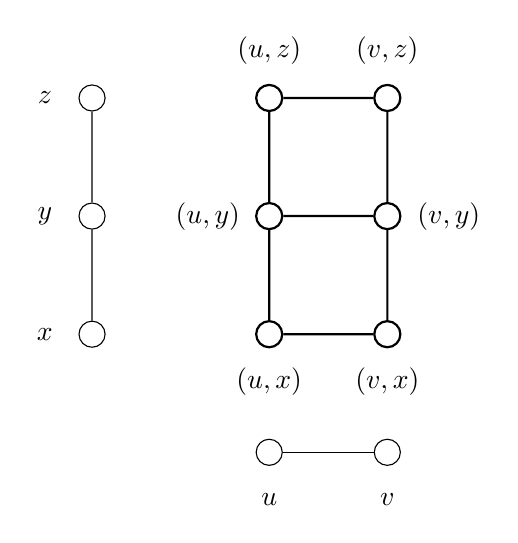
\begin{tikzpicture}[xscale=1.5, yscale=1.5]
                \tikzmath{\o = 0.4;}
                \begin{scope}[every node/.style={circle,draw}]
                \node (u) at (1,0) {};
                \node (v) at (2,0) {};
                
                \node (x) at (-0.5,1) {};
                \node (y) at (-0.5,2) {};
                \node (z) at (-0.5,3) {};
                \end{scope}
                
                \node at (1, -\o) {$u$};
                \node at (2, -\o) {$v$};
                
                \node at (-0.5-\o, 1) {$x$};
                \node at (-0.5-\o, 2) {$y$};
                \node at (-0.5-\o, 3) {$z$};
                
                \path[-,draw]
                (u) edge (v)
                (x) edge (y)
                (y) edge (z);
    
                \begin{scope}[every node/.style={circle,thick,draw}]
                \node (ux) at (1,1) {};
                \node (uy) at (1,2) {};
                \node (uz) at (1,3) {};
                \node (vx) at (2,1) {};
                \node (vy) at (2,2) {};
                \node (vz) at (2,3) {};
                \end{scope}
                
                \node at (1, 1-\o) {$(u,x)$};
                \node at (2, 1-\o) {$(v,x)$};
                \node at (1-1.3*\o, 2) {$(u,y)$};
                \node at (2+1.3*\o, 2) {$(v,y)$};
                \node at (1, 3+\o) {$(u,z)$};
                \node at (2, 3+\o) {$(v,z)$};
                
                \path[-,draw,thick]
                (ux) edge (uy)
                (uy) edge (uz)
                (vx) edge (vy)
                (vy) edge (vz)
                (ux) edge (vx)
                (uy) edge (vy)
                (uz) edge (vz);
            \end{tikzpicture}
        \end{subfigure}
        \begin{subfigure}{0.49\textwidth}
            \centering
            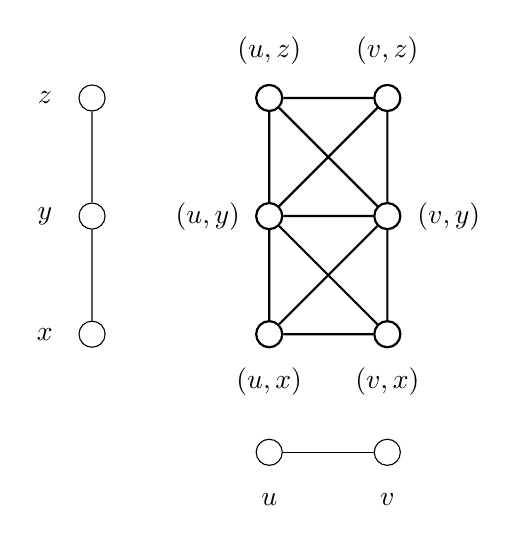
\begin{tikzpicture}[xscale=1.5, yscale=1.5]
                \tikzmath{\o = 0.4;}
                \begin{scope}[every node/.style={circle,draw}]
                \node (u) at (1,0) {};
                \node (v) at (2,0) {};
                
                \node (x) at (-0.5,1) {};
                \node (y) at (-0.5,2) {};
                \node (z) at (-0.5,3) {};
                \end{scope}
                
                \node at (1, -\o) {$u$};
                \node at (2, -\o) {$v$};
                
                \node at (-0.5-\o, 1) {$x$};
                \node at (-0.5-\o, 2) {$y$};
                \node at (-0.5-\o, 3) {$z$};
                
                \path[-,draw]
                (u) edge (v)
                (x) edge (y)
                (y) edge (z);
                
                \begin{scope}[every node/.style={circle,thick,draw}]
                \node (ux) at (1,1) {};
                \node (uy) at (1,2) {};
                \node (uz) at (1,3) {};
                \node (vx) at (2,1) {};
                \node (vy) at (2,2) {};
                \node (vz) at (2,3) {};
                \end{scope}
                
                \node at (1, 1-\o) {$(u,x)$};
                \node at (2, 1-\o) {$(v,x)$};
                \node at (1-1.3*\o, 2) {$(u,y)$};
                \node at (2+1.3*\o, 2) {$(v,y)$};
                \node at (1, 3+\o) {$(u,z)$};
                \node at (2, 3+\o) {$(v,z)$};
                
                \path[-,draw,thick]
                (ux) edge (uy)
                (uy) edge (uz)
                (vx) edge (vy)
                (vy) edge (vz)
                (ux) edge (vx)
                (uy) edge (vy)
                (uz) edge (vz)
                (ux) edge (vy)
                (uy) edge (vx)
                (uy) edge (vz)
                (uz) edge (vy);
            \end{tikzpicture}
        \end{subfigure}
        \caption{Na sliki sta prikazana kartezični produkt $P_2 \boxempty P_3$ (levo) in $P_2 \boxtimes P_3$ (desno). Kartezični produkt označujemo z $\boxempty$, krepki produkt pa z $\boxtimes$ ravno zaradi rezultata teh dveh produktov poti $P_2$ same s seboj.}
        \label{fig:produkta-poti}
    \end{figure}
    
    Pri obeh produktih opazimo, da kot inducirani podgrafi za ustrezno izbrano podmnožico vozlišč nastopajo 3 (ravno $|P_3|$) kopije grafa $P_2$ in 2 (ravno $|P_2|$) kopiji grafa $P_3$.
    
    Na spodnjih slikah je prikazan še primer kartezičnega in krepkega produkta cikla in poti na $n$ vozliščih, natančneje $C_4 \boxempty P_n$ na sliki~\ref{fig:kartez-produkt-cikel-pot} in $C_4 \boxtimes P_n$ na sliki~\ref{fig:krep-produkt-cikel-pot}.
    \begin{figure}[h]
        \centering
        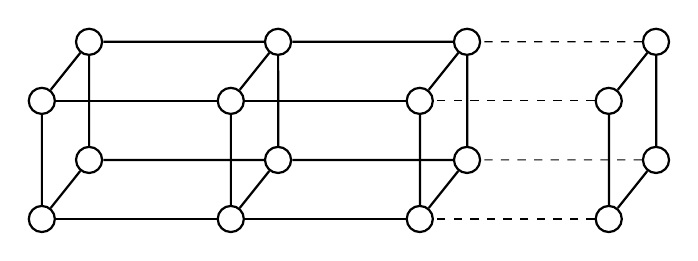
\begin{tikzpicture}[xscale=1.2,yscale=1.5]
        \foreach \i in {1,...,4}
        {
            \begin{scope}[every node/.style={circle,thick,draw}]
                \node (u\i) at (2*\i,0) {};
                \node (v\i) at (2*\i,1) {};
                \node (x\i) at (2*\i+0.5,0.5) {};
                \node (y\i) at (2*\i+0.5,1.5) {};
            \end{scope}
            
            \path[-,thick,draw]
            (u\i) edge (v\i)
            (x\i) edge (y\i)
            (u\i) edge (x\i)
            (v\i) edge (y\i);
            \ifthenelse{\i=1}{}{
                \tikzmath{\im = int(\i-1);}
                \ifthenelse{\NOT \i=4}{
                    \path[-,thick,draw]
                    (u\i) edge (u\im)
                    (v\i) edge (v\im)
                    (x\i) edge (x\im)
                    (y\i) edge (y\im);
                }{
                    \path[dashed,draw]
                    (u\i) edge (u\im)
                    (v\i) edge (v\im)
                    (x\i) edge (x\im)
                    (y\i) edge (y\im);
                }
            }
        }
        \end{tikzpicture}
        \caption{Prikazan je kartezični produkt $C_4 \boxempty P_n$.}
        \label{fig:kartez-produkt-cikel-pot}
    \end{figure}
    
    \begin{figure}[h]
        \centering
        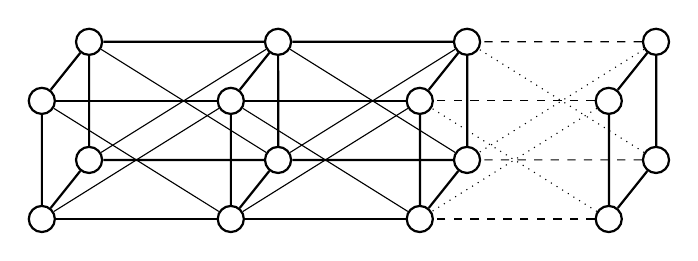
\begin{tikzpicture}[xscale=1.2,yscale=1.5]
        \foreach \i in {1,...,4}
        {
            \begin{scope}[every node/.style={circle,thick,draw}]
            \node (u\i) at (2*\i,0) {};
            \node (v\i) at (2*\i,1) {};
            \node (x\i) at (2*\i+0.5,0.5) {};
            \node (y\i) at (2*\i+0.5,1.5) {};
            \end{scope}
            
            \path[-,thick,draw]
            (u\i) edge (v\i)
            (x\i) edge (y\i)
            (u\i) edge (x\i)
            (v\i) edge (y\i);
            \ifthenelse{\i=1}{}{
                \tikzmath{\im = int(\i-1);}
                \ifthenelse{\NOT \i=4}{
                    \path[-,thick,draw]
                    (u\i) edge (u\im)
                    (v\i) edge (v\im)
                    (x\i) edge (x\im)
                    (y\i) edge (y\im);
                    \path[-,draw]
                    (u\i) edge (v\im)
                    (v\i) edge (u\im)
                    (x\i) edge (y\im)
                    (y\i) edge (x\im);
                }{
                \path[dashed,draw]
                (u\i) edge (u\im)
                (v\i) edge (v\im)
                (x\i) edge (x\im)
                (y\i) edge (y\im);
                \path[dotted,draw]
                (u\i) edge (v\im)
                (v\i) edge (u\im)
                (x\i) edge (y\im)
                (y\i) edge (x\im);
                
                }
            }
        }
        \end{tikzpicture}
        \caption{Prikazan je krepki produkt $C_4 \boxtimes P_n$.}
        \label{fig:krep-produkt-cikel-pot}
    \end{figure}
\end{primer}

Iz zgornjih definicij in primerov lahko vidimo, da sta tako kartezični kot tudi krepki produkt komutativna produkta, do izomorfnosti grafov natančno. Poglejmo si še en grafovski produkt, za katerega pa komutativnost v splošnem ne velja.

\begin{definicija}
    \emph{Korona} grafov $G$ in $H$, označimo jo z $G \circ H$, je graf velikosti $|G||H| + |G|$, ki ga sestavimo tako, da vzamemo eno kopijo $G$ in $|G|$ kopij grafa $H$, vsa vozlišča $i$-te kopije $H$ pa povežemo z $i$-tim vozliščem v kopiji grafa $G$.
\end{definicija}
Na spodnji sliki~\ref{fig:korona-poti-cikla} sta prikazani koroni $C_5 \circ P_2$ in $P_2 \circ C_5$.

\begin{figure}[h]
    \begin{subfigure}{0.33\textwidth}
        \centering
        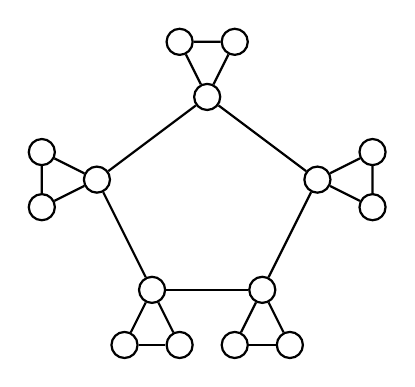
\begin{tikzpicture}[scale=0.7]
        \begin{scope}[every node/.style={circle,thick,draw}]
        \node (1) at (0,0) {};
        \node (2) at (2,0) {};
        \node (3) at (3,2) {};
        \node (4) at (1,3.5) {};
        \node (5) at (-1,2) {};
        
        \node (u1) at ([shift=({-0.5,-1})]1) {};
        \node (v1) at ([shift=({0.5,-1})]1) {};
        
        \node (u2) at ([shift=({-0.5,-1})]2) {};
        \node (v2) at ([shift=({0.5,-1})]2) {};
        
        \node (u3) at ([shift=({1,-0.5})]3) {};
        \node (v3) at ([shift=({1,0.5})]3) {};
        
        \node (u4) at ([shift=({-0.5,1})]4) {};
        \node (v4) at ([shift=({0.5,1})]4) {};
        
        \node (u5) at ([shift=({-1,-0.5})]5) {};
        \node (v5) at ([shift=({-1,0.5})]5) {};
        \end{scope}
        
        \path[-,thick,draw]
        (1) edge (2)
        (2) edge (3)
        (3) edge (4)
        (4) edge (5)
        (5) edge (1);
        
        \foreach \i in {1,...,5}
        {
            \path[-,thick,draw]
            (u\i) edge (v\i)
            (u\i) edge (\i)
            (v\i) edge (\i);
        }
        \end{tikzpicture}
    \end{subfigure}
    \begin{subfigure}{0.66\textwidth}
        \centering
        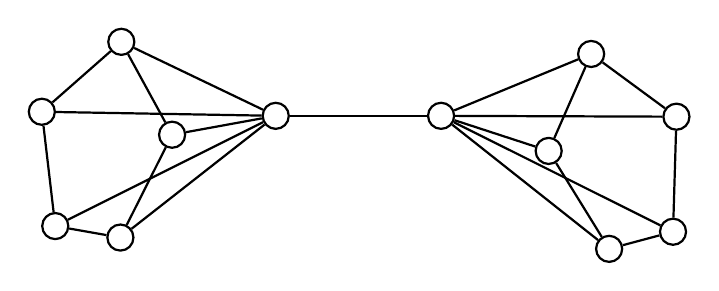
\begin{tikzpicture}[scale=0.7]
        \begin{scope}[every node/.style={circle,thick,draw}, rotate=-10, xscale=0.6]
        \node (1) at (0,0) {};
        \node (2) at (2,0) {};
        \node (3) at (3,2) {};
        \node (4) at (1,3.5) {};
        \node (5) at (-1,2) {};
        \end{scope}
        
        \begin{scope}[every node/.style={circle,thick,draw}, rotate=15, xscale=0.6, shift={(16,-3)}]
        \node (6) at (0,0) {};
        \node (7) at (2,0) {};
        \node (8) at (3,2) {};
        \node (9) at (1,3.5) {};
        \node (10) at (-1,2) {};
        \end{scope}
        
        \begin{scope}[every node/.style={circle,thick,draw}]
         \node (v1) at (4,2) {};
         \node (v2) at (7,2) {};
        \end{scope}
        
        \path[-,thick,draw]
        (1) edge (2)
        (2) edge (3)
        (3) edge (4)
        (4) edge (5)
        (5) edge (1)
        (6) edge (7)
        (7) edge (8)
        (8) edge (9)
        (9) edge (10)
        (10) edge (6)
        (v1) edge (v2);
        
        \foreach \i in {1,...,5} {
            \path[-,thick,draw]
            (\i) edge (v1);
        }
        \foreach \i in {6,...,10} {
            \path[-,thick,draw]
            (\i) edge (v2);
        }
        \end{tikzpicture}
    \end{subfigure}
    \caption{Na sliki sta prikazana korona $C_5 \circ P_2$ (levo) in $P_2 \circ C_5$ (desno). Že iz velikosti lahko vidimo, da grafa nista izomorfna.}
    \label{fig:korona-poti-cikla}
\end{figure}

\subsection{Ničelna prisila}

Poglejmo si osnovno definicijo pojmov, ki so temelji tega dela, njihove osnovne lastnosti in jih demonstrirajmo na preprostih primerih.

\begin{definicija}
    \emph{Množica ničelne prisile} $Z$ grafa $G$ je podmnožica vozlišč tega grafa, takšna, da velja: če na začetku s črno barvo pobarvamo vsa vozlišča iz $Z$, potem pa sledimo pravilu, da vsako črno vozlišče $u$ z natanko enim belim sosedom $v$ povzroči, da vozlišče $v$ spremeni barvo v črno (označimo $u \rightarrow v$), in postopek ponavljamo, dokler se še dogajajo kakšne spremembe, morajo biti po koncu postopka vsa vozlišča grafa $G$ pobarvana črno.
\end{definicija}

\begin{primer}
    \label{prim:osnovni-zf}
    Za graf na sliki~\ref{fig:osnovni-primer-prisile} je množica ničelne prisile na primer $Z = \{ 1, 5\}$. 
    \begin{figure}[h]
        \centering
        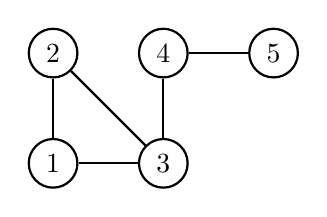
\begin{tikzpicture}[scale=0.7]
        \begin{scope}[every node/.style={circle,thick,draw}]
        \node (1) at (0,0) {1};
        \node (2) at (0,2) {2};
        \node (3) at (2,0) {3};
        \node (4) at (2,2) {4};
        \node (5) at (4,2) {5};
        \end{scope}
        
        \path[-,thick,draw]
        (1) edge (2)
        (2) edge (3)
        (1) edge (3)
        (3) edge (4)
        (4) edge (5);
        
        \end{tikzpicture}
        \caption{Ena izmed petih možnih množic ničelne prisile velikosti~2 grafa na sliki je množica $Z =\{1,5\}$.}
        \label{fig:osnovni-primer-prisile}
    \end{figure}
    Pravzaprav od podmnožic vozlišč velikosti~2 zadostujejo tiste, ki vsebujejo vozlišče~1 ali vozlišče~2 ter hkrati vozlišče~3 ali vozlišče~5, pa tudi podmnožica, ki vsebuje tako vozlišče~1 kot vozlišče~2. (Če se virus začne širiti iz trikotnika, potem morata biti pobarvani vsaj dve izmed vozlišč trikotnika, če pa se začne širiti iz vozlišča~5, ki je stopnje 1, mora biti pobarvano vsaj še eno vozlišče trikotnika (1 ali 2), da bo vozlišče~3 lahko okužilo zadnje neokuženo vozlišče trikotnika.) Vse možne množice ničelne prisile velikosti~2 so torej:
    \[ Z_1 = \{ 1, 2\}, Z_2 = \{ 1, 3\},\ Z_3 = \{ 1, 5\},\ Z_4 = \{ 2, 3\},\ Z_5 = \{2, 5\}. \]
    Če gledamo podmnožice vozlišč velikosti~3, pa so množice ničelne prisile vse, razen tista, ki ne vsebuje ne vozlišča~1 ne vozlišča~2, torej množica $\{3, 4, 5\}$. Množice ničelne prisile velikosti 4 so očitno vse možne podmnožice vozlišč velikosti 4.
\end{primer}

Zanima nas, kakšna je najmanjša možna množica vozlišč, ki jo moramo vzeti, da bo po končanem postopku barvanja celoten graf pobarvan črno. 

\begin{definicija}
    \emph{Število ničelne prisile} $Z(G)$ grafa $G$ je definirano kot velikost najmanjše množice ničelne prisile grafa $G$, oziroma
    \[ Z(G) = \min \{|Z| \mid Z \subseteq V(G) \text{ množica ničelne prisile grafa } G \}. \]
\end{definicija}

Hitro vidimo, da je število ničelne prisile dobro definirano, saj lahko za poljuben graf vedno vzamemo vsa vozlišča, razen enega, in s tem dobimo množico ničelne prisile. Velja torej
\begin{equation}
    Z(G) \leq |G| - 1.
    \label{eq:trv-zgornja-meja}
\end{equation}
Po drugi strani seveda velja tudi, da moramo za zadostitev definicije vedno imeti vsaj eno vozlišče, da lahko govorimo o množici ničelne prisile, očitno velja
\begin{equation}
Z(G)  \geq 1.
\label{eq:trv-trv-spodnja-meja}
\end{equation}
Hitro lahko postavimo boljšo očitno spodnjo mejo. Če imamo graf z najmanjšo stopnjo vozlišča $\delta$, mora biti velikost množice ničelne prisile $|Z|$ vsaj $\delta$. V nasprotnem primeru, če bi torej na začetku pobarvali $\delta - 1$ vozlišč ali manj, bi imelo vsako od pobarvanih vozlišč stopnjo vsaj $\delta$, torej bi imelo vsako od pobarvanih vozlišč $u$ vsaj $\delta - (\delta - 1 - 1) = 2$ nepobarvana soseda (ker je $u$ eno izmed pobarvanih vozlišč in ni samo svoj sosed) in se proces širjenja barve sploh ne bi mogel začeti. Velja torej spodnja meja
\begin{equation}
    Z(G) \geq \delta.
    \label{eq:trv-spodnja-meja}
\end{equation}
Ta spodnja meja je tesna za splošen graf $G$ brez dodatnih omejitev: če vzamemo primer poti $P_n$, ki ima $\delta = 1$, vidimo, da je $Z(G)$ prav tako enak 1 (pobarvamo eno od krajišč poti), torej $Z(P_n) = \delta(P_n).$

Smiselno je vprašati se, ali je ob neki začetni množici pobarvanih vozlišč $Z$, ki ni nujno množica ničelne prisile, končen rezultat postopka širjenja barve vedno enaka množica neodvisno od vrstnega reda spreminjanja barve. Pokažimo:
\begin{trditev}
    Končna množica pobarvanih vozlišč za neko začetno množico $Z$ je vedno ista, ne glede na vrstni red sprememb barv. 
\end{trditev}
\begin{proof}
    Pokažimo, da vozlišče, ki postane črno za nek vrstni red sprememb barv, lahko vedno postane črno, s pomočjo indukcije na število sprememb barv, ki so potrebne, da pobarvamo vozlišče~\cite[str.~1633]{aim2008minimumrank}. 
    
    Fiksirajmo $Z$. Recimo, da za počrnitev vozlišča $u$ potrebujemo 1 spremembo barve. To pomeni, da je $u$ edini nepobarvan sosed enega izmed vozlišč v $Z$ (sprememba barve, ki jo potrebujemo, je ravno barva vozlišča $u$). Ne glede na to, v kakšnem vrstnem redu spreminjamo barve vozlišč, bo $u$ še vedno edini nepobarvan sosed enega izmed vozlišč v $Z$ in bo nekoč pobarvan.
    
    Sedaj naj naša trditev velja za vozlišča, ki potrebujejo $n-1$ sprememb barv, da postanejo črna. Recimo, da za vozlišče $u$ potrebujemo $n$ sprememb barv. To pomeni, da obstaja sosed $v$, ki potrebuje $n-1$ sprememb barv, da počrni, pri čemer bo vozlišče $u$ po tem edini nepobarvan sosed vozlišča $v$. Ker smo predpostavili, da trditev drži za vozlišča, ki potrebujejo $n-1$ sprememb, torej velja, da bo vozlišče $v$ postalo črno neodvisno od vrstnega reda sprememb. Po nekem vrstnem redu sprememb imamo torej črno vozlišče $v$, katerega edini nepobarvan sosed je $u$, ki bo torej (nekoč) postal črn. Torej tudi za vozlišče $u$ velja, da bo postalo pobarvano neodvisno od vrstnega reda sprememb, in indukcija je zaključena.
\end{proof}

Za dano množico ničelne prisile $Z$ lahko zapišemo zaporedje sprememb barv vozlišč, pri čemer je sprememba oblike $u \rightarrow v$. Zaporedje lahko razbijemo na podzaporedja, tako da vozlišča inducirajo pot; takemu podzaporedju rečemo \emph{veriga sprememb} in ga zapišemo kot $(u_1, u_2, \ldots, u_k)$, pri čemer velja $u_i \rightarrow u_{i+1}$ za $1 \leq i \leq k-1$.  Ta podzaporedja so disjunktna (glede na vozlišča), saj vsako vozlišče povzroči spremembo v največ enem vozlišču (saj se ta zgodi, ko ima natanko enega belega soseda) in je vsako vozlišče spremenilo barvo zaradi enega vozlišča (ali pa je bilo v začetni množici $Z$). Povedano drugače, vsako vozlišče se v zaporedju sprememb nahaja največ dvakrat: enkrat na levi strani spremembe, drugič na desni. Poleg tega vemo, da se vsako vozlišče, ki ni v $Z$, v zaporedju sprememb pojavi vsaj enkrat, saj je $Z$ množica ničelne prisile in mora biti na koncu torej pobarvan cel graf. Število verig je $|Z|$, začetno vozlišče vsake so ravno vozlišča iz $Z$, pri čemer za verigo sprememb štejemo tudi eno samo vozlišče iz $Z$, če ta ne povzroči spremembe v nobenem vozlišču. Verige so torej particija vozlišč grafa, ki inducira neko pokritje s potmi. Iz tega sledi
\begin{trditev}[{\cite[trditev~2.10]{barioli2010zero}}]
    Za velikost minimalnega pokritja splošnega grafa $G$ s potmi $P(G)$ velja
    \[ P(G) \leq Z(G) .\]
\end{trditev}
Poglejmo si, kako izgleda veriga sprememb na grafu s slike~\ref{fig:osnovni-primer-prisile} iz primera~\ref{prim:osnovni-zf}, pri čemer vzemimo množico ničelne prisile $Z_3 = \{1,5\}$. Če se dogovorimo, da v primeru večih možnih povzročiteljev spremembe prevlada vozlišče z manjšo oznako, dobimo verigi $5 \rightarrow 4 \rightarrow 3$ in $1 \rightarrow 2$.

Če imamo dano množico ničelne prisile $Z$ za nek graf $G$ in v $Z$ dodamo še kakšno vozlišče, se izkaže, da je to še vedno množica ničelne prisile grafa $G$.
\begin{trditev}
    \label{trd:nadmnozica-zfs-je-zfs}
    Za graf $G$ je dana množica ničelne prisile $Z_1$. Potem za $Z_2 \subseteq V$ velja:
    \[ Z_1 \subseteq Z_2 \implies Z_2 \text{ je množica ničelne prisile} \]
\end{trditev}
\begin{proof}
    Imejmo množico ničelne prisile $Z_1$ in tako podmnožico $Z_2$ vozlišč $G$, da velja $Z_1 \subseteq Z_2$. Naj bo $z_1 = |Z_1|$ in $z_2 = |Z_2|$. Označimo zaporedje sprememb barv vozlišč, če so na začetku pobarvana vozlišča iz $Z_1$, takole: $u_1 \rightarrow v_1, u_2 \rightarrow v_2 \ldots$, pri čemer $u_i \rightarrow v_i$ pomeni, da je $u_i$ povzročil spremembo barve vozlišča $v_i$, in $i$ teče od 1 do $n - z_1$, saj je $Z_1$ množica ničelne prisile in mora biti na koncu pobarvan cel graf. Očitno je, da so vozlišča v zaporedju, ki spremenijo barvo, enolična, torej $v_i \neq v_j$ za $i \neq j$. Če sedaj na začetku pobarvamo vozlišča iz $Z_2$ in gremo po zaporedju sprememb barv za $Z_1$, imamo za spremembo $u_i \rightarrow v_i$ dve možnosti:
    \begin{itemize}
        \item $v_i$ še ni pobarvan in je edini bel sosed $u_i$ (na začetku smo dodali več črnih vozlišč, torej se je število belih sosedov vozlišč kvečjemu zmanjšalo, ne povečalo), v tem primeru se zgodi sprememba barve kot originalno;
        \item $v_i$ je že pobarvan, kar se lahko zgodi le, če $v_i \in Z_2 \setminus Z_1$, saj smo sledili spremembam barve za $Z_1$, kjer se $v_i$ pojavi samo enkrat; sprememba barve se ne zgodi.
    \end{itemize}
Druga možnost se zgodi natanko $z_2 - z_1$-krat, toliko sprememb torej ``zavržemo'', ostale pa se zgodijo kot originalno. Teh je torej $n - z_1 -(z_2 - z_1) = n - z_2$, na začetku smo pobarvali $z_2$ vozlišč, torej je zdaj skupaj pobarvanih $z_2 + n - z_2 = n$ vozlišč, $Z_2$ je torej množica ničelne prisile.
\end{proof}

Iz trditve~\ref{trd:nadmnozica-zfs-je-zfs} vidimo, da za dve množici ničelne prisile $Z_1, Z_2$ grafa $G$ velja, da je njuna unija $Z_1 \cup Z_2$ tudi množica ničelne prisile za $G$. To pa ne velja za presek: če vzamemo graf $K_2$, z vozliščema 1 in 2, sta $Z_1 = \{1\}$ in $Z_2 = \{2\}$ množici ničelne prisile, njun presek, prazna množica, pa očitno ni množica ničelne prisile za $K_2$.

Velja pa tudi naslednja posledica trditve~\ref{trd:nadmnozica-zfs-je-zfs}:
\begin{posledica}
    \label{posl:ne-obstaja-manjsi-zfs}
    Če za graf $G$ ne obstaja množica ničelne prisile velikosti $z_1$, kjer $1 < z_1 < n-1$, potem tudi ne obstaja množica ničelne prisile velikosti $z_2 < z_1$.
\end{posledica}
\begin{proof}
    Fiksirajmo $z_1$ in $z_2 \leq z_1$. Dokažimo, da če ne velja desna stran implikacije, tudi leva ne velja. Naj torej obstaja množica ničelne prisile velikosti $z_2$. Po trditvi~\ref{trd:nadmnozica-zfs-je-zfs} ji lahko dodajamo vozlišča grafa $G$, dokler ne bo velikosti $z_1$, pa bo še vedno množica ničelne prisile. Sledi torej, da obstaja množica ničelne prisile velikosti $z_1$ in dokaz je končan. 
\end{proof}

Kaj se zgodi z ničelno prisilo grafa, če odstranimo kakšno povezavo in / ali vozlišče? Če za nek graf $G$ poznamo $Z(G)$, za njegov podgraf v splošnem ne moremo povedati, kakšna bo ničelna prisila. V poglavju~\ref{sec:osnovni-rezultati} npr.~dokažemo, da ima cikel $C_n$ ničelno prisilo 2, polni graf $K_n$ pa $n-1$. V tem primeru (gledamo dovolj velike vrednosti $n$) za vpeti podgraf $C_n$ velja $Z(C_n) \leq Z(K_n)$. Če pa vzamemo kolo $W_n$ in vpet podgraf zvezdo $S_n$, pa velja $n-1 = Z(S_n) \geq Z(W_n) = 3$.

% Kaj je z induciranimi podgrafi? Če vzameš samo presek Z_G in V(H), ni nujno v redu, lahko pride prazna množica. Mogoče še naslednjega, ki se forsira? Tole ima pomoje nekaj veze s path coverjem.

Poglejmo si še, zakaj temu pojmu rečemo ``ničelna prisila''. Najprej definirajmo graf $\G(A)$ simetrične matrike $A$ velikosti $n$ nad poljem~$\F$ (pišemo $A \in Sym_n(\F)$):
\[ V(\G(A)) = \{1, \ldots n\},\ E(\G(A)) = \{\{i,j\} \mid a_{ij} \neq 0,\ 1 \leq i < j \leq n \}. \]
\begin{primer}
    Graf, ki pripada matriki \[ A = \begin{bmatrix*}[r]
    5 & -2 & 3 & 0 & 0 \\
    -2 & 13 & 6.9 & 0 & 0 \\
    3 & 6.9 & 0 & 7 & 0 \\
    0 & 0 & 7 & -1.1 & 1 \\
    0 & 0 & 0 & 1 & 0 \\
    \end{bmatrix*},\] je prikazan na sliki~\ref{fig:osnovni-primer-prisile}.
\end{primer}
Sedaj lahko definiramo množico vseh (simetričnih) matrik grafa $G$ nad poljem~$\F$:
\[ S(\F, G) = \{A \in Sym_n(\F) \mid \G(A) = G \}. \]
Ideja za imenom ničelne prisile je sledeča. Črna vozlišča predstavljajo tiste koordinate v vektorju, za katere zahtevamo, da so enake nič, bela vozlišča pa so tiste koordinate, za katere (še) ni nobene zahteve. Sprememba barve $i$-tega vozlišča iz bele v črno pomeni, da mora $i$-ta koordinata biti nič pri predpostavki, da so vse ostale koordinate, katerih vozlišča so trenutno črna, enake nič in je vektor v jedru matrike grafa $G$. Brez dokaza navedimo
\begin{trditev}[{\cite[trditev 2.3]{aim2008minimumrank}}]
    Imejmo množico ničelne prisile $Z$ grafa $G$ in matriko $A \in S(\F, G)$ grafa $G$ nad poljem $\F$. Naj bo vektor $x$ v jedru matrike $A$. Če so vse koordinate, ki pripadajo vozliščem iz $Z$, enake 0, potem je $x = 0$.
\end{trditev}


\section{Osnovni rezultati}
\label{sec:osnovni-rezultati}

V tem poglavju si ogledamo, kakšno je število ničilne prisile za nekatere osnovne družine grafov, kot npr.~poti, cikli ali polni grafi.

\subsection{Poti}
Pot dolžine $n$ je graf z $n$ vozlišči, od katerih sta dve stopnje~1 (krajišči), preostala vozlišča pa so stopnje 2. Za poti velja: 
\begin{trditev}
    $Z(P_n) = 1$.
    \label{trd:pot}
\end{trditev}
\begin{proof}
    Če na začetku pobarvamo eno izmed krajišč, označimo ga z $u$, ki je torej stopnje 1, potem ta prisili v spremembo svojega edinega soseda $v$, ki je stopnje 2 in katerega sosed $u$ je že pobarvan, zato $v$ prisili v spremembo svojega edinega nepobarvanega soseda in tako dalje \ldots (Predstavljeno tudi na sliki~\ref{fig:pot}.) Velja torej $Z(P_n) \leq 1$, saj je krajišče množica ničelne prisile. Ker je $\delta = 1$, po trivialni spodnji meji~\ref{eq:trv-spodnja-meja} velja $Z(P_n) = 1$.
    \begin{figure}[h]
        \begin{subfigure}{0.5\textwidth}
            \centering
            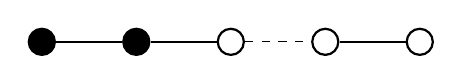
\begin{tikzpicture}[scale=1.2]
            \begin{scope}[every node/.style={circle,thick,draw}]
            \foreach \i in {1,...,5}
            {
                \ifthenelse{\i>2} {
                \node (\i) at (\i,0) {}; } {
                \node[fill=black] (\i) at (\i,0) {}; }
            }
            \end{scope}

            \foreach \i in {2,...,5}
            {
                \tikzmath{\im = int(\i-1);}
                \ifthenelse{\NOT \i=4} {
                \path[-,thick,draw]
                (\im) edge (\i); }{
                \path[dashed,draw]
                (\im) edge (\i); }
            }
            \end{tikzpicture}
        \end{subfigure}
        \begin{subfigure}{0.49\textwidth}
            \centering
            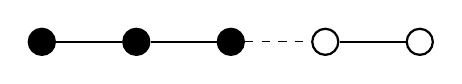
\begin{tikzpicture}[scale=1.2]
            \begin{scope}[every node/.style={circle,thick,draw}]
            \foreach \i in {1,...,5}
            {
                \ifthenelse{\i>3} {
                    \node (\i) at (\i,0) {}; } {
                    \node[fill=black] (\i) at (\i,0) {}; }
            }
            \end{scope}
            
            \foreach \i in {2,...,5}
            {
                \tikzmath{\im = int(\i-1);}
                \ifthenelse{\NOT \i=4} {
                    \path[-,thick,draw]
                    (\im) edge (\i); }{
                    \path[dashed,draw]
                    (\im) edge (\i); }
            }
            \end{tikzpicture}
        \end{subfigure}
        \caption{Prikazano je vmesno stanje širjenja črne barve v grafu $P_n$, če smo na začetku pobarvali samo levo krajišče. Drugo vozlišče z leve ima natanko enega nepobarvanega soseda (na sliki levo) in ga prisili v spremembo barve (na sliki desno). Širjenje se nadaljuje na enak način, dokler ni pobarvan cel graf.}
        \label{fig:pot}
    \end{figure}
\end{proof}

\subsection{Cikli}
Cikel na $n$ vozliščih $C_n$ je graf, v katerem imajo vsa vozlišča stopnjo~2, velja torej $\delta = \Delta = 2$.
\begin{trditev}
    $Z(C_n) = 2$. 
\end{trditev}
\begin{figure}[h]
    \begin{subfigure}{0.5\textwidth}
        \centering
        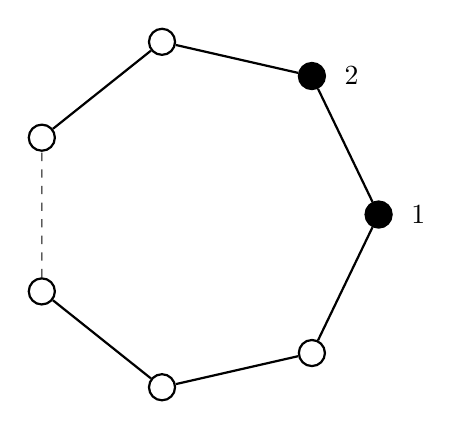
\begin{tikzpicture}[scale=0.9]
        \tikzmath{\n = 7; \r = 2.5;}
        \begin{scope}[every node/.style={circle,thick,draw}]
        \foreach \i in {1,...,\n}
        {
            \ifthenelse{\i>2} {
                \node (\i) at ({360/\n * (\i - 1)}: \r) {}; } {
                \node[fill=black, label=right:{\i}] (\i) at ({360/\n * (\i - 1)}: \r) {}; }
        }
        \end{scope}
        
        \foreach \i in {1,...,\n}
        {
            \tikzmath{\im = int(mod(\i,\n)+1);}
            \ifthenelse{\NOT \i=4} {
                \path[-,thick,draw]
                (\im) edge (\i); }{
                \path[dashed,draw]
                (\im) edge (\i); }
        }
        \end{tikzpicture}
    \end{subfigure}
    \begin{subfigure}{0.49\textwidth}
        \centering
        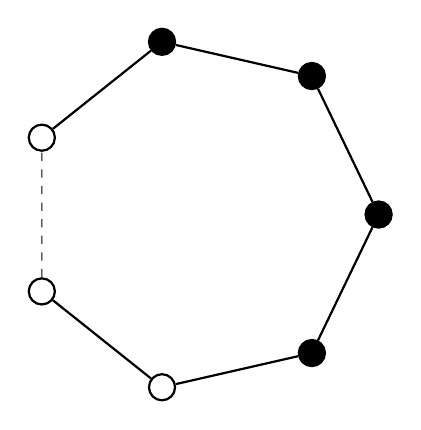
\begin{tikzpicture}[scale=0.9]
        \tikzmath{\n = 7; \r = 2.5;}
        \begin{scope}[every node/.style={circle,thick,draw}]
        \foreach \i in {1,...,\n}
        {
            \ifthenelse{\i>3 \AND \i<\n} {
                \node (\i) at ({360/\n * (\i - 1)}: \r) {}; } {
                \node[fill=black] (\i) at ({360/\n * (\i - 1)}: \r) {}; }
        }
        \end{scope}
        
        \foreach \i in {1,...,\n}
        {
            \tikzmath{\im = int(mod(\i,\n)+1);}
            \ifthenelse{\NOT \i=4} {
                \path[-,thick,draw]
                (\im) edge (\i); }{
                \path[dashed,draw]
                (\im) edge (\i); }
        }
        \end{tikzpicture}
    \end{subfigure}
    \caption{Prikazano je vmesno stanje širjenja barve v grafu $C_n$, pri čemer sta na začetku pobarvani sosednji vozlišči~1 in~2 (prikazano na sliki levo). Vozlišče~1 lahko v spremembo prisili desnega soseda, vozlišče~2 pa levega soseda (prikazano na sliki desno). Postopek se ponavlja, dokler ni pobarvan cel graf.}
    \label{fig:cikel}
\end{figure}
\begin{proof}
    Če za začetno množico pobarvanih vozlišč vzamemo dva soseda, bo vsak imel natanko enega nepobarvanega soseda, širjenje bo torej potekalo v obe smeri (prikazano na sliki~\ref{fig:cikel}), dokler ne bo cel graf pobarvan. Takšna začetna množica torej je množica ničelne prisile, torej velja $Z(C_n) \leq 2$. Če upoštevamo trivialno spodnjo mejo~\ref{eq:trv-spodnja-meja} in dejstvo, da je najmanjša stopnja v ciklu enaka~2, dobimo $Z(C_n) = 2$.\qedhere
\end{proof}

\subsection{Polni grafi}
Polni graf na $n$ vozliščih $K_n$ je graf, v katerem je vsako vozlišče sosednje vsem ostalim, vsa vozlišča so torej stopnje $n-1$. 
\begin{trditev}
    \label{trd:polni-graf}
    $Z(K_n) = n-1$.
\end{trditev}
\begin{proof}
    Če pobarvamo vsa vozlišča, razen enega (označimo $v$), je to množica ničelne prisile, saj so vsi sosedi vozlišča $v$ črni in je $v$ njihov edini nepobarvan sosed, torej ga prisilijo v spremembo barve in pobarvan je cel graf. Velja torej $Z(K_n) \leq n-1$, po spodnji meji~\ref{eq:trv-spodnja-meja} pa velja tudi $Z(K_n) \geq \delta = n-1$, torej je $Z(K_n) = n-1$.
\end{proof}
Na sliki~\ref{fig:polni-graf} je prikazan polni graf na 5 vozliščih in njegova množica ničelne prisile.
\begin{figure}[h]
    \centering
    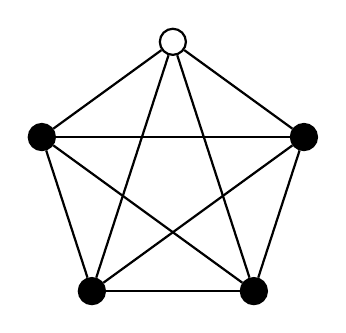
\begin{tikzpicture}[scale=0.7]
    \tikzmath{\n = 5; \r = 2.5; \nm = int(\n-1);}
    \begin{scope}[every node/.style={circle,thick,draw}]
    \foreach \i in {1,...,\n}
    {
        \ifthenelse{\i<2} {
            \node (\i) at ({90 + (360/\n * (\i - 1))}: \r) {}; } {
            \node[fill=black] (\i) at ({90 + (360/\n * (\i - 1))}: \r) {}; }
    }
    \end{scope}
    
    \foreach \i in {1,...,\nm}
    {
        \tikzmath{\ip = int(\i + 1);}
        \foreach \j in {\ip,...,\n} {
            \path[-,thick,draw] (\i) edge (\j); 
        }
    }
    \end{tikzpicture}
    \caption{Prikazan je polni graf $K_5$ in njegova množica ničelne prisile. Čim bi pobarvali eno vozlišče manj, bi imelo vsako črno vozlišče dva nepobarvana soseda in se postopek širjenja barve ne bi mogel začeti.}
    \label{fig:polni-graf}
\end{figure}

\subsection{Zvezde}
Zvezda $S_n$ je tak graf na $n+1$ vozliščih, ki ima $n$ vozlišč stopnje~1 in eno vozlišče stopnje~$n$. Je pravzaprav poseben primer polnega dvodelnega grafa, množico vozlišč lahko torej razbijemo na dve množici $X$, v kateri je vozlišče stopnje $n$, in $Y$, v kateri so vsa preostala vozlišča, ki so stopnje 1. Znotraj množic $X$ in $Y$ ni povezav, vsako vozlišče iz $X$ pa je sosednje vsakemu v $Y$. Primer zvezde je prikazan na sliki~\ref{fig:zvezda}.
\begin{figure}[h]
    \centering
    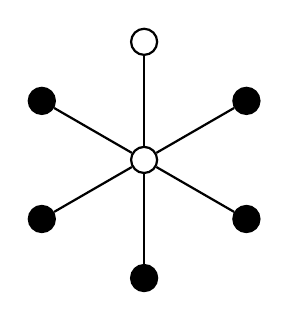
\begin{tikzpicture}[scale=0.6]
    \tikzmath{\n = 6; \r = 2.5; \nm = int(\n-1);}
    \begin{scope}[every node/.style={circle,thick,draw}]
    \foreach \i in {1,...,\n} {
        \ifthenelse{\i<2} {
            \node (\i) at ({90 + (360/\n * (\i - 1))}: \r) {}; } {
            \node[fill=black] (\i) at ({90 + (360/\n * (\i - 1))}: \r) {}; }
    }
    \node (0) at (0,0) {};
    \end{scope}
    
    \foreach \i in {1,...,\n} {
        \path[-,thick,draw] (\i) edge (0); 
    }
    \end{tikzpicture}
    \caption{Prikazana je zvezda $S_6$ in njena množica ničelne prisile.}
    \label{fig:zvezda}
\end{figure}

\begin{trditev}
    $Z(S_n) = n - 1$.
\end{trditev}
\begin{proof}
    Za namene tega dokaza si bomo sliko zvezde predstavljali kot poln dvodelen graf $K_{1,n}$ (podobno kot na sliki~\ref{fig:polni-dvodelni-graf}), sredinsko vozlišče stopnje $n$ na eni strani (množica $X$), na drugi pa vsa preostala vozlišča, ki so stopnje 1 (množica $Y$).
    Opazimo, da so vozlišča iz $Y$ ekvivalentna v smislu, da ni važno, katero točno je pobarvano, saj imajo vsa isto stopnjo in soseda. Če črno pobarvamo vsa vozlišča v $Y$ razen enega, bo eno izmed teh vozlišč poskrbelo za spremembo barve sredinskega vozlišča stopnje $n$, to pa bo poskrbelo za spremembo barve edinega vozlišča stopnje 1, ki še ni črno. Velja torej $Z(K_{1,n}) \leq n-1$. Poskusimo najti manjšo množico ničelne prisile. Na začetku lahko pobarvamo $n-2$ vozlišča na dva načina: lahko pobarvamo vozlišče stopnje $n$ in $n-3$ vozlišč stopnje 1, lahko pa pobarvamo $n-2$ vozlišč stopnje 1. Obravnavajmo oba primera.
    \begin{enumerate}[a)]
        \item Če na začetku pobarvamo vozlišče stopnje $n$ in $n-3$ vozlišč stopnje 1, potem črna vozlišča stopnje 1 nimajo več nobenega nepobarvanega soseda, vozlišče stopnje $n$ pa ima še 3 nepobarvane sosede, zato se črna barva ne more širiti. 
        \item Če na začetku pobarvamo $n-2$ vozlišč stopnje 1, ima vsako od njih enega nepobarvanega soseda, to je vozlišče stopnje $n$, ki torej spremeni barvo. Sedaj ima vozlišče stopnje $n$ še 2 nepobarvana soseda in širjenje barve se ustavi.
    \end{enumerate}
    Torej ne glede na to, kako izberemo začetno množico velikosti $n-2$, ta ne bo množica ničelne prisile. Velja torej $Z(S_n) = n-1$.
\end{proof}

\subsection{Polni dvodelni grafi}
Poln dvodelni graf $K_{m,n}$ je tak graf na $m+n$ vozliščih, kjer lahko množico vozlišč razbijemo na dve množici $V_m$ velikosti $m$ in $V_n$ velikosti $n$ tako, da znotraj vsake od množic ni povezav, vsako vozlišče iz $V_m$ pa je sosednje vsakemu vozlišču iz $V_n$. Na sliki~\ref{fig:polni-dvodelni-graf} je prikazan primer polnega dvodelnega graf $K_{3,4}$.
\begin{figure}[h]
    \centering
    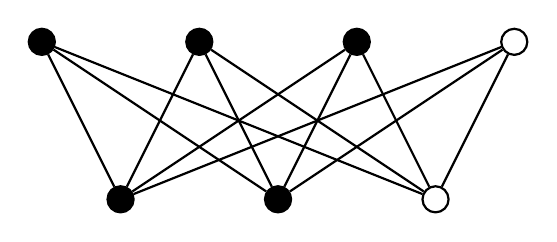
\begin{tikzpicture}
    \tikzmath{\n = 4; \m = 3;}
    \begin{scope}[every node/.style={circle,thick,draw}]
    \foreach \i in {1,...,\m} {
        \ifthenelse {\i < \m} {
            \node[fill=black] (u\i) at (1+2*\i, 0) {}; }{
            \node (u\i) at (1+2*\i, 0) {}; }
    }
    \foreach \i in {1,...,\n} {
        \ifthenelse {\i < \n} {
            \node[fill=black] (v\i) at (2*\i, 2) {}; }{
            \node (v\i) at (2*\i, 2) {}; }
    }
    \end{scope}
    
    \foreach \i in {1,...,\m} {
        \foreach \j in {1,...,\n} {
            \path[-,thick,draw] (u\i) edge (v\j); 
        }
    }
    \end{tikzpicture}
    \caption{Prikazan je polni dvodelni graf $K_{3,4}$ in njegova množica ničelne prisile.}
    \label{fig:polni-dvodelni-graf}
\end{figure}
\begin{trditev}
    \label{trd:polni-dvodelni-graf}
    $Z(K_{m,n}) = m + n - 2$.
\end{trditev}
\begin{proof}
    Če je $m=1$, dobimo ravno zvezdo, $Z(K_{1,n}) = 1 + n - 2 = n - 1 = Z(S_n)$, trditev torej velja.
    
    Zdaj si poglejmo splošen primer, torej število ničelne prisile $K_{m,n}$. Če na začetku pobarvamo $m-1$ vozlišč iz $V_m$ in $n-1$ vozlišč iz $V_n$, lahko eno izmed pobarvanih vozlišč v $V_m$ prisili v spremembo barve edino nepobarvano vozlišče v $V_n$ in obratno. Velja torej $Z(K_{m,n}) \leq (m - 1) + (n - 1) = m + n -2$. Sedaj poskusimo najti $m + n - 3$ vozlišč, ki so množica ničelne prisile. Podobno kot v posebenem primeru zvezde jih lahko izberemo tako, da pobarvamo vsa vozlišča iz $V_n$ in $m-3$ vozlišč iz $V_m$, v tem primeru pobarvana vozlišča iz $V_m$ nimajo nobenega nepobarvanega soseda, vozlišča iz $V_n$ pa imajo tri nepobarvane sosede, zato se barva ne more razširiti. Simetrično v primeru, če pobarvamo vsa vozlišča iz $V_m$ in $n-3$ vozlišč iz $V_n$. Če na začetku pobarvamo $m-1$ vozlišč iz $V_m$ in $n-2$ vozlišč iz $V_n$, potem imajo črna vozlišča iz $V_n$ enega nepobarvanega soseda, ki torej spremeni barvo, pobarvana vozlišča iz $V_m$ pa imajo 2~nepobarvana soseda, torej se širjenje ustavi. Simetrično, če na začetku pobarvamo $m-2$ vozlišč iz $V_m$ in $n-1$ vozlišč iz $V_n$. Ne glede na to, kako izberemo vozlišča, torej ne dobimo množice ničelne prisile. Velja torej $Z(K_{m,n}) \geq m + n - 2$, trditev sledi.
\end{proof}

\subsection{Kolesa}
Kolo $W_n$ je graf na $n+1$ vozliščih, ki ga dobimo, če vzamemo cikel $C_n$, na sredino postavimo še eno vozlišče in ga povežemo z vsemi ostalimi. Najmanjša stopnja v grafu je torej $\delta = 3$, največja pa $\Delta = n$. Kolo $W_7$ je prikazano na sliki~\ref{fig:kolo}.
\begin{figure}[h]
    \centering
    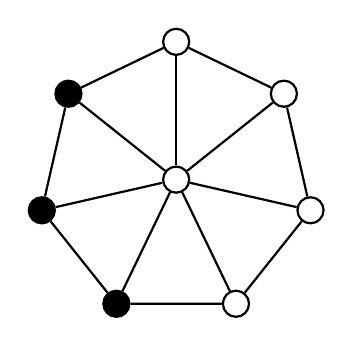
\begin{tikzpicture}[scale=0.7]
        \tikzmath{\n = 7; \r = 2.5; \nm = int(\n-1);}
        \begin{scope}[every node/.style={circle,thick,draw}]
        \foreach \i in {1,...,\n} {
            \ifthenelse{\i<2 \OR \i>4 } {
                \node (\i) at ({90 + (360/\n * (\i - 1))}: \r) {}; } {
                \node[fill=black] (\i) at ({90 + (360/\n * (\i - 1))}: \r) {}; }
        }
        \node (0) at (0,0) {};
        \end{scope}
        
        \foreach \i in {1,...,\n} {
            \tikzmath{\im = int(mod(\i,\n)+1);}
            \path[-,thick,draw] (\i) edge (0); 
            \path[-,thick,draw] (\i) edge (\im); 
        }
    \end{tikzpicture}
    \caption{Na sliki je prikazano kolo $W_7$ in njegova množica ničelne prisile.}
    \label{fig:kolo}
\end{figure}
\begin{trditev}
    $Z(W_n) = 3$.
\end{trditev}
\begin{proof}
    Če na začetku pobarvamo enega izmed vozlišč stopnje 3, označimo ga z $u$, in njegova soseda, označimo ju z $v$ in $w$, potem ima $u$ natanko enega nepobarvanega soseda, to je sredinsko vozlišče, ki torej postane črno. Sedaj ima $v$ natanko enega nepobarvanega soseda $x$, saj sta sredinsko vozlišče in $u$ že pobarvana. Tudi $x$ ima nato natanko enega nepobarvanega soseda, saj sta sredinsko vozlišče in $v$ že črna. Postopek se nadaljuje, podobno se dogaja tudi z druge strani (z vozliščem $w$ in njegovimi sosedi), na koncu so pobarvana vsa vozlišča. Velja torej $Z(W_n) \leq 3$, po trivialni spodnji meji~\ref{eq:trv-spodnja-meja} pa velja tudi $Z(W_n) \geq \delta = 3$, trditev sledi.
\end{proof}

\subsection{Trikotniki}
Trikotnik $T_n$ je graf z $\frac{n (n+1)}{2}$ vozlišči. Najlažje ga definiramo rekurzivno:
$T_1$ je graf na enem vozlišču (tudi $K_1$), graf $T_n$ pa iz grafa $T_{n-1}$ dobimo tako, da pod sliko grafa $T_{n-1}$ dodamo $n$ vozlišč v ravni vrsti, jih povežemo v pot, nato pa vsako vozlišče povežemo z vozliščema iz prejšnje ravni, ki imata enak indeks ali indeks, ki je za ena večji. Zapišimo matematično: če $j$-to vozlišče na $i$-ti ravni označimo z $u_{i,j}$, potem za graf $T_n$ velja: 
\begin{align*}
    V(T_n) &= \{u_{i,j} \mid i=0,\ldots,n-1, \quad j=0,\ldots,i \} \\
    E(T_n) &= \{ \{u_{i,j}, u_{i, j+1} \} \mid i=1,\ldots,n-1, \quad j=0,\ldots,i-1  \} 
    \\ &\phantom{=} \cup \{ \{ u_{i-1, j}, u_{i,j}  \} \mid i=1,\ldots,n-1, \quad j=0,\ldots,i-1  \} 
    \\ &\phantom{=} \cup \{ \{ u_{i-1, j},u_{i,j+1} \} \mid i=1,\ldots,n-1, \quad j=0,\ldots,i-1  \} 
\end{align*}
Za lažjo predstavo je na sliki~\ref{fig:trikotnik} prikazan primer grafa $T_4$ skupaj z oznakami vozlišč.
\begin{figure}[h]
    \centering
    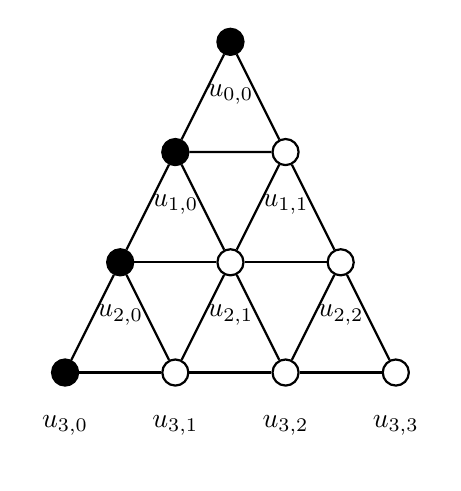
\begin{tikzpicture}[scale=0.7]
    \tikzmath{\n = 4; \nm = \n-1;}
    \begin{scope}[every node/.style={circle,thick,draw}]
    \foreach \i in {0,...,\nm} {
        \tikzmath{\z = int(\nm - \i);}
        \foreach \j in {0,...,\i} {
            \ifthenelse{\j=0}{
                \node[fill=black,label=below:{$u_{\i,\j}$}] (\i\j) at (\z + 2*\j, 2*\z) {};
            }{
                \node[label=below:{$u_{\i,\j}$}] (\i\j) at (\z + 2*\j, 2*\z) {};
            }
        }
    }
    \end{scope}
    
    \foreach \i in {1,...,\nm} {
        \tikzmath{\im = int(\i-1);}
        \foreach \j in {0,...,\im} {
            \tikzmath{\jv = int(\j+1); \jm = int(\j-1);}
            \path[-,thick,draw] (\i\j) edge (\im\j); 
            \path[-,thick,draw] (\i\j) edge (\i\jv); 
            \path[-,thick,draw] (\i\jv) edge (\im\j);
        }
    }
    \end{tikzpicture}
    \caption{Prikazan je trikotnik $T_4$ in ena izmed njegovih množic ničelne prisile.}
    \label{fig:trikotnik}
\end{figure}

\begin{trditev}
    $Z(T_n) = n$. 
\end{trditev}
\begin{proof}
    Na začetku pobarvajmo eno izmed stranic trikotnika (npr.~levo, kot na sliki~\ref{fig:trikotnik}, torej vozlišča $u_{i,0}$ za $i = 0, \ldots, n-1$). Vozlišče $u_{0,0}$ ima natanko enega nepobarvanega soseda, to je diagonalni sosed $u_{1,1}$, ki torej postane črn. Nato ima $u_{1,0}$ natanko enega nepobarvanega soseda, to je $u_{2,1}$, ki spremeni barvo, in zato ima $u_{2,0}$ natanko enega nepobarvanega soseda in tako naprej \ldots Tako se barva razširi po celi diagonali, pobarvana so torej tudi vsa vozlišča $u_{i,1}$ za $i = 1, \ldots, n-1$. Sedaj ima $u_{1,1}$ natanko enega nepobarvanega soseda, to je $u_{2,2}$, nato ima $u_{2,1}$ natanko enega nepobarvanega soseda $u_{3,2}$, barva se ponovno razširi po celi diagonali $u_{i,2}$ za $i = 2, \ldots, n-1$. Postopek se ponavlja, na koncu se barva razširi na vse diagonale $u_{i,j},\ i = j, \ldots, n-1$ za $j = 1, \ldots, n-1$, torej na vsa vozlišča grafa $T_n$. Velja torej $Z(T_n) \leq n$.
    
    \hl{TODO: večje enako in posledično enakost}
\end{proof}

\subsection{Drevesa?}

\section{Ekstremni primeri}
Poglejmo si, za katere grafe je pri zgornji~\eqref{eq:trv-zgornja-meja} in trivialni spodnji~\eqref{eq:trv-trv-spodnja-meja} meji za ničelno prisilo dosežena enakost. 
\begin{trditev}
    Za graf $G$ na $n > 1$ vozliščih velja:
    \[ Z(G) = n - 1 \iff G = K_n .\]
    Z besedami, enakost v zgornji meji~\eqref{eq:trv-zgornja-meja} je dosežena natanko takrat, ko imamo polni graf na $n$ vozliščih.
\end{trditev}
\begin{proof}
    Po trditvi~\ref{trd:polni-graf} vemo, da velja implikacija v levo, torej
    \[ G = K_n \implies Z(G) = n-1. \]
    S protislovjem dokažimo še implikacijo v desno, vzemimo torej graf $G$, za katerega velja $Z(G) = n-1$. Recimo, da graf $G$ ni polni graf, torej obstaja neko vozlišče $u$, katerega stopnja je strogo manjša od $n-1$. 
    Dokažimo najprej, da iz tega sledi, da obstaja vozlišče $w$, ki je sosed enega izmed sosedov $u$, ni pa tudi sosed $u$-ja. Če tako vozlišče $w$ ne bi obstajalo, bi (zaradi predpostavke povezanosti) to pomenilo, da je naš celoten graf sestavljen iz $u$ in njegovih sosedov, je torej graf na $n = \deg(u) + 1$ vozliščih, vozlišče $u$ pa ima stopnjo $\deg(u) = n-1$, kar je v nasprotju s predpostavko.
    
    Množico ničelne prisile lahko sedaj sestavimo tako, da pobarvamo vse sosede $u$, razen enega, poleg tega pa še vsa preostala vozlišča v grafu, razen vozlišča $w$. Vozlišče $u$ torej povzroči spremembo barve v edinem nepobarvanem sosedu, nato pa so pobarvana že vsa vozlišča v grafu, razen $w$, ki spremeni barvo zaradi enega izmed svojih sosedov. Našli smo torej množico ničelne prisile velikosti $n-2$, kar je v protislovju s predpostavko. Sledi, da je $G = K_n$. 
\end{proof}

\begin{trditev}
    Za graf $G$ na $n$ vozliščih velja: 
    \[ Z(G) = 1 \iff G = P_n. \]
    Z besedami, enakost v trivialni spodnji meji~\eqref{eq:trv-trv-spodnja-meja} je dosežena natanko takrat, ko imamo pot na $n$ vozliščih.
\end{trditev}
\begin{proof}
    Iz trditve~\ref{trd:pot} vemo, da drži implikacija v levo. Dokažimo še implikacijo v desno, vzemimo graf $G$ na $n$ vozliščih, za katerega velja $Z(G) = 1$. Vzemimo vozlišče $u$, ki predstavlja množico ničelne prisile. Če je $n = 1$, imamo torej graf $P_1$, trditev drži. Sicer mora $u$ povzročiti vsaj eno spremembo barve, torej mora imeti natanko enega nepobarvanega soseda $v$ -- vozlišče $u$ je torej stopnje 1. Če je $n=2$, je $v$ prav tako vozlišče stopnje 1, imamo graf $P_2$ in trditev drži.  V nasprotnem primeru mora $v$ povzročiti vsaj eno spremembo barve, torej ima natanko enega nepobarvanega soseda $w$ (poleg $u$, ki je že črne barve) -- $v$ je torej stopnje 2. Če je $n=3$, je vozlišče $w$ stopnje 1, dobimo torej graf $P_3$. Sicer se postopek nadaljuje, v vsakem koraku ugotovimo, da mora biti vozlišče, ki je nazadnje spremenilo barvo, stopnje 1, če je pobarvan že ves graf, imamo torej pot na $n$ vozliščih, ali pa stopnje 2, če imamo še kakšno nepobarvano vozlišče. Širjenje barve se nekoč ustavi, saj je $n$ končen.
\end{proof}

\begin{trditev}[{\cite[izrek~2.3]{row2012technique}}]
    \hl{TODO: ?}
    \[ Z(G) = 2 \iff G \text{ je graf dveh paralelnih poti}.  \]
\end{trditev}

\section{Ničelna prisila produktov grafov}
V tem poglavju si bomo ogledali nekaj rezultatov o številu ničelne prisile za produkte grafov. Osnova za to poglavje je predvsem~\cite{aim2008minimumrank}.

\begin{trditev}
    \label{trd:kartezicni-produkt-zgornja-meja}
    Za kartezični produkt grafov $G$ in $H$ velja
    \begin{equation}
        Z(G \boxempty H) \leq \min\{Z(G) |H|, Z(H) |G|\}.
        \label{eq:kartezicni-produkt-zgornja-meja}
    \end{equation}
\end{trditev}
\begin{proof}
    Po definiciji kartezičnega produkta vemo, da graf $G \boxempty H$ vsebuje (kot podgrafe) $|H|$ kopij grafa $G$. V vsaki kopiji $G$ pobarvamo pripadajoča vozlišča, ki tvorijo množico ničelne prisile v osnovnem grafu $G$. (Natančneje, če je $U \subseteq V(G)$ množica ničelne prisile osnovnega grafa $G$, potem v grafu $G \boxempty H$ vzamemo vsa taka vozlišča, katere prva koordinata je v množici $U$.) To je množica ničelne prisile celotnega produkta, saj se širjenje barve zgodi v vsaki kopiji neodvisno, ker so po definiciji kartezičnega produkta med kopijami $G$ povezave le med vozlišči z enako prvo komponento (na začetku velja, da če je pobarvano vozlišče v eni kopiji $G$, potem so pobarvana tudi pripadajoča vozlišča v vseh ostalih kopijah $G$, ko se barva začne širiti, pa si lahko predstavljamo, da vsa istoležna vozlišča v vseh kopijah $G$ hkrati postanejo črna). Velja torej
    \[ Z(G \boxempty H) \leq Z(G) |H|, \]
    saj imamo ravno $|H|$ kopij $G$.
    
    Podobno graf $G \boxempty H$ vsebuje $|G|$ kopij grafa $H$, množico ničelne prisile konstruiramo kot prej in dobimo 
    \[ Z(G \boxempty H)  \leq Z(H) |G|, \]
    trditev sledi.
\end{proof}

Na sliki~\ref{fig:zf-kartezicni-produkt} sta prikazani množici ničelne prisile, konstruirani kot v dokazu zgornje trditve, za kartezični produkt $C_4 \boxempty P_n$. 
\begin{figure}[h]
    \begin{subfigure}{0.5\textwidth}
        \centering
        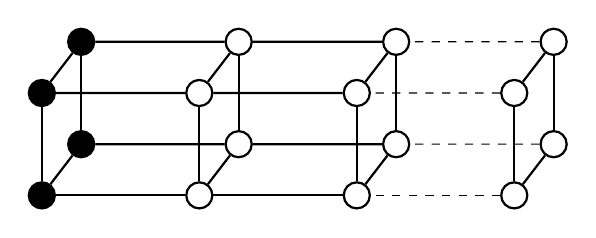
\begin{tikzpicture}[yscale=1.3]
            \foreach \i in {1,...,4}
            {
                \begin{scope}[every node/.style={circle,thick,draw}]
                \ifthenelse{\i=1}{
                    \node[fill=black] (u\i) at (2*\i,0) {};
                    \node[fill=black] (v\i) at (2*\i,1) {};
                    \node[fill=black] (x\i) at (2*\i+0.5,0.5) {};
                    \node[fill=black] (y\i) at (2*\i+0.5,1.5) {};
                    }{
                    \node (u\i) at (2*\i,0) {};
                    \node (v\i) at (2*\i,1) {};
                    \node (x\i) at (2*\i+0.5,0.5) {};
                    \node (y\i) at (2*\i+0.5,1.5) {};
                }                
                \end{scope}
                
                \path[-,thick,draw]
                (u\i) edge (v\i)
                (x\i) edge (y\i)
                (u\i) edge (x\i)
                (v\i) edge (y\i);
                \ifthenelse{\i=1}{}{
                    \tikzmath{\im = int(\i-1);}
                    \ifthenelse{\NOT \i=4}{
                        \path[-,thick,draw]
                        (u\i) edge (u\im)
                        (v\i) edge (v\im)
                        (x\i) edge (x\im)
                        (y\i) edge (y\im);
                    }{
                    \path[dashed,draw]
                    (u\i) edge (u\im)
                    (v\i) edge (v\im)
                    (x\i) edge (x\im)
                    (y\i) edge (y\im);
                }
            }
        }
        \end{tikzpicture}
    \end{subfigure}
    \begin{subfigure}{0.49\textwidth}
        \centering
        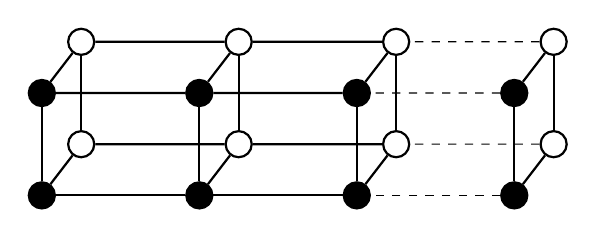
\begin{tikzpicture}[yscale=1.3]
        \foreach \i in {1,...,4}
        {
            \begin{scope}[every node/.style={circle,thick,draw}]
                \node[fill=black] (u\i) at (2*\i,0) {};
                \node[fill=black] (v\i) at (2*\i,1) {};
                \node (x\i) at (2*\i+0.5,0.5) {};
                \node (y\i) at (2*\i+0.5,1.5) {};       
            \end{scope}
            
            \path[-,thick,draw]
            (u\i) edge (v\i)
            (x\i) edge (y\i)
            (u\i) edge (x\i)
            (v\i) edge (y\i);
            \ifthenelse{\i=1}{}{
                \tikzmath{\im = int(\i-1);}
                \ifthenelse{\NOT \i=4}{
                    \path[-,thick,draw]
                    (u\i) edge (u\im)
                    (v\i) edge (v\im)
                    (x\i) edge (x\im)
                    (y\i) edge (y\im);
                }{
                    \path[dashed,draw]
                    (u\i) edge (u\im)
                    (v\i) edge (v\im)
                    (x\i) edge (x\im)
                    (y\i) edge (y\im);
                }
            }
        }
        \end{tikzpicture}
    \end{subfigure}
    \caption{Prikazan je graf $C_4 \boxempty P_n$ in množici ničelne prisile, konstruirani kot v dokazu trditve~\ref{trd:kartezicni-produkt-zgornja-meja}. Levo je množica ničelne prisile, konstruirana tako, da smo pobarvali pripadajoča vozlišča iz množice ničelne prisile grafa $P_n$ v vseh kopijah $P_n$, desno pa tako, da smo pobarvali množico ničelne prisile v vsaki kopiji $C_4$.}
    \label{fig:zf-kartezicni-produkt}
\end{figure}

Sledi nekaj trivialnih posledic trditve~\ref{trd:kartezicni-produkt-zgornja-meja}.
\begin{posledica}
    Za kartezične produkte splošnega grafa $G$ velja:
    \begin{enumerate}
        \item $Z(G \boxempty P_n) \leq \min \{ Z(G)n, |G| \} \stackrel{|G| \leq n}{=} |G|$
        \item $Z(G \boxempty C_n) \leq \min \{ Z(G)n, 2|G| \}$
        \item $Z(G \boxempty K_n) \leq \min \{ Z(G)n, (n-1)|G| \}$
    \end{enumerate}
\end{posledica}
\begin{proof}
    Pri vseh točkah uporabimo zgornjo mejo~\eqref{eq:kartezicni-produkt-zgornja-meja}, dejstvo, da so velikosti grafov $P_n, C_n$ in $K_n$ enake $n$ in rezultate o njihovih ničelnih prisilah iz poglavja~\ref{sec:osnovni-rezultati}. Dodatek pri produktu s potjo $P_n$ sledi iz trivialne spodnje meje $Z(G) \geq 1$ in predpostavke, da je $|G| \leq n$. 
\end{proof}

V posebnem, če imamo kartezični produkt dveh polnih grafov, lahko zgornjo mejo še malo izboljšamo. Po trditvi~\ref{eq:kartezicni-produkt-zgornja-meja} je zgornja meja za ničelno prisilo grafa $K_m \boxempty K_n$, predpostavimo tudi $m \leq n$, enaka $\min \{(m-1)\cdot n, (n-1) \cdot m\} = \min \{ mn - n , mn - m\} \stackrel{m \leq n}{=} m (n-1) $, torej če v vseh $m$ kopijah grafa $K_n$ pobarvamo vsa vozlišča razen enega. Vendar pa imamo še vedno množico ničelne prisile, če pobarvamo vsa vozlišča v eni kopiji $K_n$ in v $m-2$ kopijah vsa, razen enega (istoležnega v vseh kopijah), kar je ravno množica ničelne prisile znotraj te kopije, zadnjo kopijo pa pustimo belo. Za lažjo predstavo je na sliki~\ref{fig:zf-kartezicni-produkt-polnih} prikazana tako konstruirana množica ničelne prisile za produkt $K_3 \boxempty K_4$.
\begin{figure}[h]
    \centering
    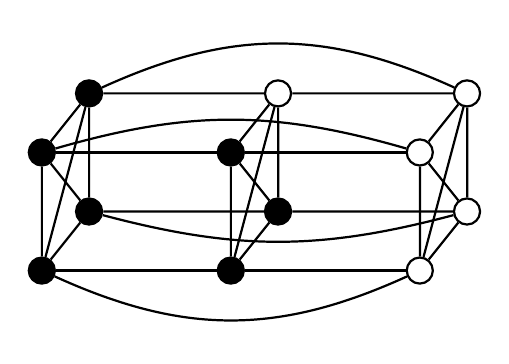
\begin{tikzpicture}[yscale=1.5, xscale=1.2]
    \foreach \i in {1,...,3}
    {
        \begin{scope}[every node/.style={circle,thick,draw}]
        \ifthenelse{\i<3}{
            \node[fill=black] (u\i) at (2*\i,0) {};
            \node[fill=black] (v\i) at (2*\i,1) {};
            \node[fill=black] (x\i) at (2*\i+0.5,0.5) {};
            \ifthenelse{\i=1}{
                \node[fill=black] (y\i) at (2*\i+0.5,1.5) {}; 
            }{
            \node (y\i) at (2*\i+0.5,1.5) {}; 
        }
    }{
    \node (u\i) at (2*\i,0) {};
    \node (v\i) at (2*\i,1) {};
    \node (x\i) at (2*\i+0.5,0.5) {};
    \node (y\i) at (2*\i+0.5,1.5) {};
}                
\end{scope}

\path[-,thick,draw]
(u\i) edge (v\i)
(x\i) edge (y\i)
(u\i) edge (x\i)
(v\i) edge (y\i)
(u\i) edge (y\i)
(v\i) edge (x\i);
\ifthenelse{\i=1}{}{
    \tikzmath{\im = int(\i-1);}
    \path[-,thick,draw]
    (u\i) edge (u\im)
    (v\i) edge (v\im)
    (x\i) edge (x\im)
    (y\i) edge (y\im);
    
}
}
\path[-,thick,draw]
(u1) edge[bend right=20] (u3)
(x1) edge[bend right=12] (x3)
(v1) edge[bend left=13] (v3)
(y1) edge[bend left=20] (y3);
\end{tikzpicture}
\caption{Prikazan je kartezični produkt $K_3 \boxempty K_4$ in množica ničelne prisile, konstruirana po trditvi~\ref{trd:kartezicni-produkt-zgornja-meja-polni}.}
\label{fig:zf-kartezicni-produkt-polnih}
\end{figure}

Poglejmo, da je to res množica ničelne prisile. Popolnoma pobarvana kopija $K_n$ bo povzročila spremembo barve v vseh vozliščih nepobarvane kopije, razen v tistem vozlišču, ki v večini kopij ni pobarvan. Nato lahko znotraj vsake kopije $K_n$ katerokoli pobarvano vozlišče spremeni barvo edinemu nepobarvanemu vozlišču v tej kopiji. Dokazali smo:
\begin{trditev}
    \label{trd:kartezicni-produkt-zgornja-meja-polni}
    $Z(K_m \boxempty K_n) \leq n + (n-1)(m-2) = m n - m - n + 2$.
\end{trditev}

Zgornja meja~\eqref{eq:kartezicni-produkt-zgornja-meja} nam da tudi zgornjo mejo za hiperkocke. \emph{Hiperkocka} velikosti $n+1$ je graf, ki ga dobimo kot kartezični produkt manjše hiperkocke velikosti $n$ in polnega grafa velikosti 2. S simboli $Q_{n+1} = Q_n \boxempty K_2$, pri čemer je $Q_0$ enak $K_1$. Na sliki~\ref{fig:hiperkocke} so prikazane hiperkocke $Q_1$, $Q_2$ in $Q_3$.
\begin{figure}[h]
    \begin{subfigure}{0.33\textwidth}
        \centering
        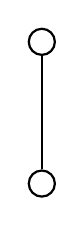
\begin{tikzpicture}[scale=0.9]
        \begin{scope}[every node/.style={circle,thick,draw}]
        \node (1) at (0,0) {};
        \node (2) at (0,2) {};  
        \end{scope}
        
        \path[-,thick,draw]
        (1) edge (2);
        \end{tikzpicture}
    \end{subfigure}
    \begin{subfigure}{0.33\textwidth}
        \centering
        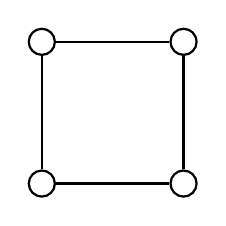
\begin{tikzpicture}[scale=0.9]
            \begin{scope}[every node/.style={circle,thick,draw}]
            \node (1) at (0,0) {};
            \node (2) at (2,0) {};
            \node (3) at (2,2) {};
            \node (4) at (0,2) {};  
            \end{scope}
            
            \path[-,thick,draw]
            (1) edge (2)
            (2) edge (3)
            (3) edge (4)
            (4) edge (1);
        \end{tikzpicture}
    \end{subfigure}
    \begin{subfigure}{0.3\textwidth}
        \centering
        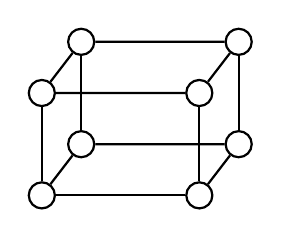
\begin{tikzpicture}[yscale=1.3]
        \foreach \i in {1,...,2}
        {
            \begin{scope}[every node/.style={circle,thick,draw}]
            \node (u\i) at (2*\i,0) {};
            \node (v\i) at (2*\i,1) {};
            \node (x\i) at (2*\i+0.5,0.5) {};
            \node (y\i) at (2*\i+0.5,1.5) {};
            \end{scope}
            
            \path[-,thick,draw]
            (u\i) edge (v\i)
            (x\i) edge (y\i)
            (u\i) edge (x\i)
            (v\i) edge (y\i);
            \ifthenelse{\i=1}{}{
                \tikzmath{\im = int(\i-1);}
                \path[-,thick,draw]
                    (u\i) edge (u\im)
                    (v\i) edge (v\im)
                    (x\i) edge (x\im)
                    (y\i) edge (y\im);
            }
        }
        \end{tikzpicture}
    \end{subfigure}
\caption{Na sliki so prikazane hiperkocke $Q_1 = K_2$ (levo), $Q_2 = K_2 \boxempty K_2 \cong C_4$ (v sredini) in $Q_3 = Q_2 \boxempty K_2 = C_4 \boxempty K_2$ (desno).}
\label{fig:hiperkocke}
\end{figure}
\begin{posledica}
    $Z(Q_n) \leq 2^{n-1}$.
\end{posledica}
\begin{proof}
    Uporabimo splošno zgornjo mejo za kartezični produkt~\eqref{eq:kartezicni-produkt-zgornja-meja} in definicijo hiperkocke. Dobimo
    \[
        Z(Q_n) = Z(Q_{n-1} \boxempty K_2) \leq \min \{ 2Z(Q_{n-1}), |Q_{n-1}| \} \leq |Q_{n-1}| = 2^{n-1},
    \]
    pri čemer upoštevamo še $|Q_{n}| = 2^n$.
\end{proof}
V hiperkocki $Q_n$ je torej dovolj, če pobarvamo eno izmed kopij manjše hiperkocke $Q_{n-1}$ (to je očitno množica ničelne prisile, saj ima vsako vozlišče v kopiji natanko enega nepobarvanega soseda, to je istoležno vozlišče v drugi kopiji).

% TODO: polni, cikel, pot s polnim, ciklom, potjo - ali imamo kakšne boljše meje

Poglejmo si še zgornjo mejo za krepki produkt poti.
\begin{trditev}
    $Z(P_m \boxtimes P_n) \leq m + n -1$.
\end{trditev}
\begin{proof}
    \begin{figure}[h]
        \begin{subfigure}{0.5\textwidth}
            \centering
            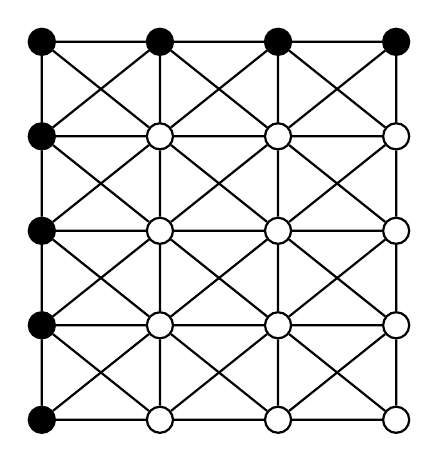
\begin{tikzpicture}[yscale=1.2, xscale=1.5]
                \tikzmath{\n = 5; \m = 4;}
                \foreach \j in {1,...,\n}
                {
                    \foreach \i in {1,...,\m}
                    {
                        \begin{scope}[every node/.style={circle,thick,draw}]
                        \ifthenelse{\i = 1 \OR \j = \n}{
                            \node[fill=black] (x\i y\j) at (\i,\j) {};
                        }{
                        \node (x\i y\j) at (\i,\j) {};
                    }
                    \end{scope}
                    \tikzmath{\jm = int(\j-1); \im = int(\i-1); \iv = int(\i+1);}
                    \ifthenelse{\i = 1 \OR \j = 1}{}{
                        \path[-,thick,draw](x\i y\j) edge (x\im y\jm);
                    }
                    \ifthenelse{\i = 1}{}{
                        \path[-,thick,draw] (x\i y\j) edge (x\im y\j);
                    }
                    \ifthenelse{\j = 1 \OR \i = \m}{}{
                        \path[-,thick,draw] (x\i y\j) edge (x\iv y\jm);
                    }
                    \ifthenelse{\j = 1}{}{
                        \path[-,thick,draw] (x\i y\j) edge (x\i y\jm);
                    }
                }
            }
            \end{tikzpicture}
        \end{subfigure}
        \begin{subfigure}{0.49\textwidth}
            \centering
            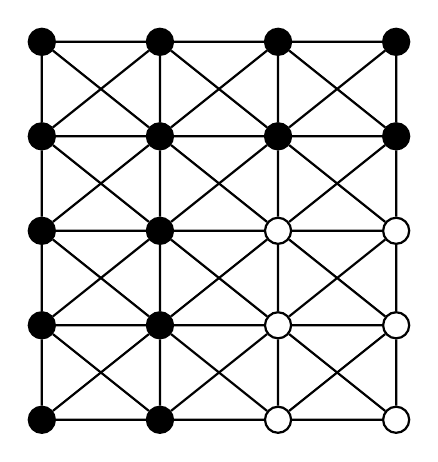
\begin{tikzpicture}[yscale=1.2, xscale=1.5]
                \tikzmath{\n = 5; \m = 4;}
                \foreach \j in {1,...,\n}
                {
                    \foreach \i in {1,...,\m}
                    {
                        \begin{scope}[every node/.style={circle,thick,draw}]
                        \tikzmath{\nm = \n - 2;}
                        \ifthenelse{\i < 3 \OR \j > \nm}{
                            \node[fill=black] (x\i y\j) at (\i,\j) {};
                        }{
                        \node (x\i y\j) at (\i,\j) {};
                    }
                    \end{scope}
                    \tikzmath{\jm = int(\j-1); \im = int(\i-1); \iv = int(\i+1);}
                    \ifthenelse{\i = 1 \OR \j = 1}{}{
                        \path[-,thick,draw](x\i y\j) edge (x\im y\jm);
                    }
                    \ifthenelse{\i = 1}{}{
                        \path[-,thick,draw] (x\i y\j) edge (x\im y\j);
                    }
                    \ifthenelse{\j = 1 \OR \i = \m}{}{
                        \path[-,thick,draw] (x\i y\j) edge (x\iv y\jm);
                    }
                    \ifthenelse{\j = 1}{}{
                        \path[-,thick,draw] (x\i y\j) edge (x\i y\jm);
                    }
                }
            }
            \end{tikzpicture}
        \end{subfigure}
        \caption{Prikazan je krepki produkt $P_4 \boxtimes P_5$, na sliki levo njegova množica ničelne prisile, na sliki desno pa vmesno stanje širjenja barve.}
        \label{fig:zf-krepki-produkt-poti}
    \end{figure}
    
    Pobarvajmo vsa vozlišča ene izmed robnih kopij $P_m$ in ene izmed robnih kopij $P_n$ (prikazano na sliki~\ref{fig:zf-krepki-produkt-poti} na primeru $P_4 \boxtimes P_5$), začetno množico pobarvanih vozlišč označimo z $Z$. Pobarvali smo ravno $m + n - 1$ vozlišč, saj je eno vozlišče, označimo ga z $u$, skupno obema kopijama. Dokažimo, da je to res množica ničelne prisile. Vozlišče $u$ je edino, ki ima natanko enega nepobarvanega soseda (diagonalnega), ki torej spremeni barvo. Sedaj ima sosed $u$ v kopiji $P_m$ natanko enega nepobarvanega soseda, diagonalnega, ki spremeni barvo, in tako naprej po celotni robni kopiji $P_m$. Simetrično pa se zgodi tudi v robni kopiji $P_n$. Po koncu je pobarvana robna in še sosednja kopija $P_m$ ter robna in sosednja kopija $P_n$, kot prikazano na sliki~\ref{fig:zf-krepki-produkt-poti} desno. Vidimo, da je trenutna situacija zelo podobna začetni. Če pogledamo induciran graf iz vozlišč $V(P_m \boxtimes P_n) \setminus Z$, vidimo, da je izomorfen grafu $P_{m-1} \boxtimes P_{n-1}$, pri čemer sta trenutno pobarvani ravno robna kopija $P_{m-1}$ in robna kopija $P_{n-1}$. Širjenje barve se torej rekurzivno nadaljuje kot prej, na koncu je pobarvan cel graf, začetna množica $Z$ je res množica ničelne prisile. 
\end{proof}

% TODO: krepki produkt, vse isto probaj

Znana je tudi zgornja meja za ničelno prisilo korone dveh splošnih grafov.
\begin{trditev}
    Za splošna grafa $G$ in $H$ velja
    \begin{align*}
        Z(G \circ H) &\leq Z(H) |G|+ Z(G) |H| - Z(G) Z(H) \\
        &= Z(H) (|G| - Z(G)) + Z(G) |H|.
    \end{align*} 
    V posebnem, če $m \geq 2$, za korono polnih grafov velja $Z(K_m \circ K_n) \leq mn - 1$. 
\end{trditev}
\begin{proof}
    Vzemimo minimalno množico ničelne prisile grafa $G$ in jo označimo z $Z_G$. Pobarvamo vozlišča v vseh tistih kopijah $H$, ki so povezane z vozliščem iz $Z_G$, s tem smo pobarvali $|Z_G| |H| = Z(G) |H|$ vozlišč, saj je $Z_G$ minimalna množica ničelne prisile za $G$. V preostalih $|G| - Z(G)$ kopijah $H$ pa pobarvamo tista vozlišča, ki tvorijo minimalno množico ničelne prisile za $H$. Vse skupaj smo torej pobarvali $Z(H)(|G| - Z(G)) + Z(G) |H|$ vozlišč. Primer tako konstruirane množice je prikazan na sliki~\ref{fig:zf-korona}.
    \begin{figure}[h]
        \centering
        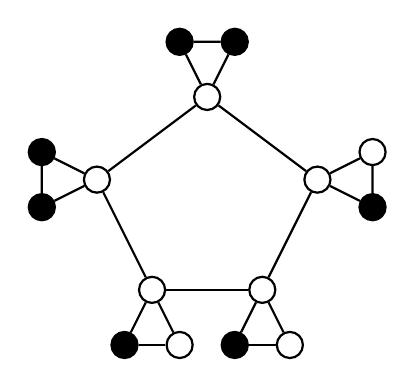
\begin{tikzpicture}[scale=0.7]
        \begin{scope}[every node/.style={circle,thick,draw}]
        \node (1) at (0,0) {};
        \node (2) at (2,0) {};
        \node (3) at (3,2) {};
        \node (4) at (1,3.5) {};
        \node (5) at (-1,2) {};
        
        \node[fill=black] (u1) at ([shift=({-0.5,-1})]1) {};
        \node (v1) at ([shift=({0.5,-1})]1) {};
        
        \node[fill=black] (u2) at ([shift=({-0.5,-1})]2) {};
        \node (v2) at ([shift=({0.5,-1})]2) {};
        
        \node[fill=black] (u3) at ([shift=({1,-0.5})]3) {};
        \node (v3) at ([shift=({1,0.5})]3) {};
        
        \node[fill=black] (u4) at ([shift=({-0.5,1})]4) {};
        \node[fill=black] (v4) at ([shift=({0.5,1})]4) {};
        
        \node[fill=black] (u5) at ([shift=({-1,-0.5})]5) {};
        \node[fill=black] (v5) at ([shift=({-1,0.5})]5) {};
        \end{scope}
        
        \path[-,thick,draw]
        (1) edge (2)
        (2) edge (3)
        (3) edge (4)
        (4) edge (5)
        (5) edge (1);
        
        \foreach \i in {1,...,5}
        {
            \path[-,thick,draw]
            (u\i) edge (v\i)
            (u\i) edge (\i)
            (v\i) edge (\i);
        }
        \end{tikzpicture}
        \caption{Prikazana je korona $C_5 \circ K_2$ in njegova množica ničelne prisile, konstruirana kot v zgornjem dokazu.}
        \label{fig:zf-korona}
    \end{figure}
    
    Poglejmo, da smo res konstruirali množico ničelne prisile. Kopije $H$, ki so popolnoma pobarvane, spremenijo barvo svojemu vozlišču iz kopije $G$. Sedaj so v $G$ torej pobarvana vsa vozlišča iz $Z_G$. Ker je $Z_G$ množica ničelne prisile za $G$ in ker so kopije $H$, povezane s temi vozlišči, že črne, ima eno izmed vozlišč v $G$ natanko enega nepobarvanega soseda v $G$. Ko ta počrni, se barva spremeni tudi vsem nepobarvanem vozliščem v njegovi kopiji $H$, saj je bila pred tem v tej kopiji pobarvana ravno množica ničelne prisile. Ker je $Z_G$ množica ničelne prisile, se ta postopek ponavlja, dokler ni pobarvan celoten graf. 
    
    Zgornja meja za korono polnih grafov v večino primerih sledi iz dokazane splošne zgornje meje (upoštevamo osnovni rezultat o ničelni prisili za polne grafe~\ref{trd:polni-graf}):
    \[ Z(K_m \circ K_n) \leq n-1 + (m-1)n = mn - 1, \text{ za } n \geq 2.\]
    Če pa je $n = 1$, nam zaradi dejstva $Z(K_1) = 1$ splošni dokaz da $1 + (m-1) = m$ namesto v trditvi želene meje $m - 1$. Konstruirajmo množico ničelne prisile velikosti $m-1$ za primer $K_m \circ K_1$ tako, da pobarvamo vse kopije $K_1$, razen ene. Pobarvane kopije $K_1$ povzročijo spremembo vsaka v svojem vozlišču kopije $K_m$, sedaj je pobarvana množica ničelne prisile v $K_m$. Eno izmed pobarvanih vozlišč spremeni barvo edinemu nepobarvanemu v $K_m$, ta pa nato povzroči še spremembo barve svoje kopije $K_1$.
\end{proof}

\section{Izračun ničelne prisile}
V tem poglavju bomo problem ničelne prisile preučili skozi stališče računske zahtevnosti: pogledali si bomo algoritem, ki preveri, ali je dana množica za dan graf res množica ničelne prisile, in s tem dokazali, da problem spada v NP. Analizirali bomo trivialen splošni algoritem za izračun ničelne prisile poljubnega grafa, si pogledali njegove potencialne izboljšave in povzeli nekaj rezultatov o NP-polnosti problema.

\subsection{Predstavitve grafov in računska zahtevnost}
Preden začnemo z analizo algoritmov, sis oglejmo načine predstavitve grafov v računalnikih in zahtevnosti operacij pri različnih predstavitvah. 

Predpostavljali bomo, da so oznake vozlišč grafa $G$ velikosti $n$ kar cela števila od 0 do $n-1$ (v večini programskih jezikov indeks v seznamih in podobnih podatkovnih strukturah teče od 0 naprej). Zaradi takih oznak pri delu z grafi lahko uporabljamo eno bolj preprostih podatkovnih struktur, seznam, saj si podatek o $i$-tem vozlišču (npr.~barvo) shranimo pod indeks~$i$. Če so oznake kaj drugega in jih bomo kasneje potrebovali, jih lahko preslikamo v števila od 0 do $n-1$ in si v seznam na $i$-to mesto shranimo prejšnjo oznako vozlišča. 

Prvi način predstavitve je matrika sosednosti. Ta vsebuje ničle na tistih indeksih $(i,j)$, za katere velja, da vozlišči $i$ in $j$ nista sosednji, in enke za tista vozlišča, ki so sosednja. Na diagonali so torej vedno ničle, saj graf ne vsebuje zank, v primeru neusmerjenega grafa pa je matrika še simetrična. Predstavimo jo s seznamom seznamov, $i$-ti element zunanjega seznama je $i$-ta vrstica matrike, torej porabimo $O(n^2)$ prostora. Kakšna je zahtevnost pogostih operacij nad grafom? Da ugotovimo, ali sta vozlišči $i$ in $j$ sosednji, porabimo $O(1)$, saj moramo le preveriti, ali je element v $i$-ti vrstici na $j$-tem indeksu ena, in je dostop do elementa seznama prek indeksa časovne zahtevnosti $O(1)$. Enako časovno zahtevnost ima iz istega razloga tudi dodajanje ali odstranjevanje povezave. Če želimo poiskati vse sosede vozlišča $i$, porabimo $O(n)$, saj moramo preveriti celotno $i$-to vrstico. Če želimo dodati ali odstraniti vozlišče, potrebujemo $O(2n)$ operacij (gremo čez en stolpec in eno vrstico), pri čemer pri odstranjevanju v večini primerih porabimo še več, saj brisanje elementa iz seznama v najslabšem primeru traja $O(n)$, medtem ko je dodajanje na konec seznama amortizirano $O(1)$.

Graf lahko predstavimo tudi s seznamom sosedov: za vsako vozlišče naštejemo njegove sosede. V tem primeru prav tako uporabimo seznam seznamov, pri čemer se na indeksu~$i$ zunanjega seznama nahaja seznam sosedov vozlišča $i$. Pri tem porabimo $O(n+m)$ prostora, kjer je $m = |E|$ število povezav grafa. Če nas zanima, ali sta vozlišči $i$ in $j$ sosednji, moramo pregledati celoten seznam sosedov vozlišča~$i$, torej je časovna zahtevnost enaka $O(\deg i)$. Če je seznam urejen, lahko uporabimo binarno iskanje, ki ima logaritmično časovno zahtevnost, torej $O(\log \deg i)$. Odstranjevanje povezave med vozliščema $i$ in $j$ traja $O(2 \deg i + 2 \deg j)$, saj moramo v seznamu sosedov obeh poiskati in odstraniti drugo vozlišče, pri iskanju moramo v najslabšem primeru preiskati cel seznam sosedov, pri odstranjevanju pa ga prekopirati eno v levo. V najslabšem primeru traja celotna operacija $O(4n)$ (če je seznam sosedov urejen, pa $O(2\log n + 2n)$). Dodajanje povezave $ij$ traja $O(1)$, če nam vrstni red seznama sosedov ni pomemben. Če pa nam je vrstni red pomemben, lahko na seznamu sosedov $i$ in $j$ uporabimo binarno iskanje, da najdemo pravo mesto. V tem primeru porabimo $O(\log \deg i + \deg i)$ za eno vozlišče, saj ima dodajanje v seznam dolžine $p$ časovno zahtevnost $O(p)$, v najslabšem primeru skupaj torej $O(2 \log n + 2 n)$. Da najdemo vse sosede nekega vozlišča, moramo le pogledati na $i$-to mesto zunanjega seznama, torej ima operacija konstantno časovno zahtevnost. Če želimo dodati vozlišče, moramo dodati seznam z njegovimi sosedi na konec zunanjega seznama in njegovo oznako na konec nekaterih seznamov sosedov, kar traja $O(n)$. Za odstranjevanje vozlišča pa moramo odstraniti njegov seznam sosedov in vozlišče odstraniti iz vseh ostalih seznamov sosedov. Za prvo porabimo $O(n)$, za drugo pa $O(n^2)$, skupna časovna zahtevnost je torej $O(n^2)$.

Seznam sosedov lahko implementiramo tudi kot seznam množic. Če so te implementirane z zgoščenimi tabelami, to pomeni, da imajo preverjanje, ali je element v množici, dodajanje in odstranjevanje v povprečju konstantno časovno zahtevnost. Ali sta vozlišči sosednji, lahko zato ugotovimo v konstantnem času, prav toliko porabimo tudi za odstranjevanje povezave in dodajanje povezave. Dodajanje vozlišča je še vedno $O(n)$, odstranjevanje pa prav tako postane $O(n)$. 

Vse tri predstavitve lahko primerjamo v tabeli~\ref{tab:primerjava-predstavitev}.
Na prvi pogled se zdi, da bi bilo vedno najbolj optimalno izbrati seznam sosedov, implementiran z množicami. Vendar pa je treba upoštevati, da dodajanje, iskanje in odstranjevanje iz množice v povprečju sicer je konstantne časovne zahtevnosti, je pa ta konstanta večja kot npr.~pri dodajanju na konec seznama. Tako je predstavitev najbolj smiselno izbrati glede na to, katere operacije bomo potrebovali in koliko prostora imamo na voljo oziroma kako velike grafe želimo obravnavati. 

\begin{table}[h]
    \centering
    \begin{tabular}{lccc}
        \toprule
        & matrika sosednosti & seznam sosedov (s) & seznam sosedov (m) \\ \midrule
        prostor & $O(n^2)$ & $O(n + m)$ & $O(n + m)$ \\
        $i \sim j$ & $O(1)$ & $O(n)$ & $O(1)$ \\
        dodaj $e = ij$ & $O(1)$ & $O(1)$ & $O(1)$ \\
        odstrani $e = ij$ & $O(1)$ & $O(n)$ & $O(1)$ \\
        vsi sosedi $i$ & $O(n)$ & $O(1)$ & $O(1)$\\
        dodaj $i$ & $O(2n)$ & $O(n)$ & $O(n)$ \\
        odstrani $i$ & $O(n^2)$ & $O(n^2)$ & $O(n)$ \\
        \bottomrule
    \end{tabular}
    \caption{Prikazana je primerjava časovnih zahtevnosti nekaterih pogostih operacij na grafih med tremi predstavitvami: matrika sosednosti (2.~stolpec), seznam sosedov, implementiran s seznamom (3.~stolpec) in seznam sosedov, implementiran z množico (4.~stolpec).}
    \label{tab:primerjava-predstavitev}
\end{table}

Ker se bomo dotaknili tudi težavnosti odločitvenih problemov, si poglejmo nekaj osnovnih definicij računske zahtevnosti.
\begin{definicija}
    \begin{enumerate}
        \item Odločitveni problem $\Pi$ spada v razred \P, pišemo $\Pi \in \P$, če ga lahko rešimo z determinističnim Turingovim strojem s polinomsko časovno zahtevnostjo.
        \item Odločitveni problem $\Pi$ spada v razred \NP, pišemo $\Pi \in \NP$, če ga lahko rešimo z nedeterminističnim Turingovim strojem s polinomsko časovno zahtevnostjo.
    \end{enumerate}
\end{definicija}
Povedano drugače, v razred $\P$ spadajo tisti problemi, za katere poznamo algoritem, ki najde rešitev v polinomskem času. Po drugi strani v $\NP$ spadajo tisti problemi, za katere poznamo algoritem, ki v polinomskem času preveri, ali je dana rešitev pravilna. Spodnja definicija razreda $NP$ je namreč ekvivalentna zgornji \hl{TODO citat}:
\begin{definicija}
    Problem $\Pi$ je v $\NP$, če obstaja certifikat, polinomske dolžine glede na vhodne podatke, za rešitev in obstaja polinomski algoritem (preverjevalec), ki vrne ``da'', če certifikat za konkreten primer problema dokaže, da je odgovor na problem ``da'', in ``ne'' sicer.
\end{definicija}

Hitro vidimo, da velja $\P \subseteq \NP$. Če za problem poznamo algoritem, ki najde rešitev v polinomskem času, potem moramo poznati tudi algoritem, ki v polinomskem času preveri pravilnost te rešitve, saj sicer ne moremo biti gotovi, da nam prvi algoritem res vrne rešitev problema. (Isto lahko vidimo tudi iz zgornjih definicij obeh razredov, saj je deterministični Turingov stroj posebna različica nedeterminističnega Turingovega stroja.)

Ali velja tudi $\NP \subseteq \P$ in posledično $\P = \NP$? To bi pomenilo, da je vsak problem, katerega rešitev lahko preverimo v polinomskem času, tudi rešljiv v polinomskem času. Odgovor na vprašanje ni znan, veliko matematikov pa predvideva, da je nikalen, saj po nekaj desetletjih preučevanja težkih problem znotraj $\NP$, rečemo jim tudi $\NP$-polni, znanih naj bi jih bilo več kot 3000~\cite{wikiPvsNP}, nihče ni uspel najti polinomskega algoritma za kateregakoli izmed njih.

\begin{definicija}
    \label{def:np-poln}
    Odločitveni problem $\Pi$ je \emph{$\NP$-poln}, pišemo $\Pi \in \NPC$, če velja:
    \begin{enumerate}
        \item $\Pi \in \NP$,
        \item vsak problem $\Pi' \in \NP$ lahko v polinomskem času prevedemo na $\Pi$.
    \end{enumerate}
\end{definicija}
Polinomska prevedljivost problema $\Pi'$ na problem $\Pi$ pomeni, da je reševanje $\Pi'$ lažje (oziroma kvečjemu polinomsko težje) od reševanja problema $\Pi$. Povedano drugače, nek algoritem, ki reši problem $\Pi$ lahko uporabimo kot del relativno preprostega algoritma, ki reši $\Pi'$. 

Povedali smo že, da za probleme v $\NPC$ ne poznamo polinomskih algoritmov. Če bi tak algoritem za nek $\NP$-poln problem obstajal, bi sledilo $\P = \NP$:
\begin{trditev}
    Naj bo $\Pi \in \NPC$. Potem velja:
    \[ \Pi \in \P \iff \P = \NP. \]
\end{trditev}
\begin{proof}
    Implikacija v levo je očitna: če $\P = \NP$, potem $\Pi \in \NPC \implies \Pi \in \NP = \P$.
    Poglejmo še implikacijo v desno. Ker $\Pi \in \NPC$, pomeni, da lahko vsak problem v $\NP$ v polinomskem času prevedemo na $\Pi$. Ker $\Pi \in \P$, imamo polinomski algoritem za reševanje $\Pi$, torej lahko v polinomskem času rešimo tudi vse ostale probleme iz $\NP$, torej za vsak problem iz $\NP$ sledi da je tudi iz $\P$. Velja torej $\NP \subseteq \P$ in skupaj z $\P \subseteq \NP$ sledi $\P = \NP$.
\end{proof}

Problemi, ki so $\NP$-polni, so iz teorije grafov na primer problem vozliščnega pokritja, obstoja Hamiltonskega cikla in popolnega trirazsežnega prirejanja. Če želimo dokazati, da je nek problem $\NP$-poln, se tega lahko lotimo s pomočjo naslednje leme:
\begin{lema}
    Naj bo $\Pi' \in \NPC$, $\Pi \in \NP$ in naj bo $\Pi'$ v polinomskem času prevedljiv na problem $\Pi$. Potem velja $\Pi \in \NPC$.
\end{lema}
\begin{proof}
    Ker je $\Pi' \in \NPC$, lahko vsak problem iz $\NP$ v polinomskem času prevedemo na $\Pi'$. Ker lahko $\Pi'$ v polinomskem času prevedemo na $\Pi$, lahko po tranzitivnosti relacije prevedljivosti vsak problem iz $\NP$ prevedemo na $\Pi$ v polinomskem času, torej velja $\Pi \in \NPC$.
\end{proof}
$\NP$-polnost problema pa lahko dokažemo tudi tako, da ga zožimo na nek podproblem, za katerega vemo, da je $\NP$-poln. (Če je podproblem težek, potem je gotovo težek tudi širši problem.)
Ti dve tehniki bomo uporabili v podpoglavju~\ref{subsec:np-polnost}.

Do zdaj smo govorili samo o težavnosti odločitvenih problemov, kaj pa, če imamo nek splošen računski problem? Formalno definiramo, da je računski problem \emph{$\NP$-težek}, če bi obstoj polinomskega algoritma impliciral, da je $\P = \NP$. Tako sem spadajo tudi vsi $\NP$-polni (odločitveni) problemi. Če imamo nek optimizacijski problem, kot ga bomo srečali v tem delu, ga lahko prevedemo na odločitven problem; če je ta $\NP$-poln, potem je originalni problem $\NP$-težek.

\subsection{Preverljivost}
Dan imamo graf $G$ in neko podmnožico njegovih vozlišč $Z \subseteq V$. Najti želimo algoritem, ki preveri, ali je $Z$ množica ničelne prisile. To naredimo tako, da simuliramo postopek širjenja barve po pravilu, da črno vozlišče povzroči spremembo barve v edinemu nepobarvanemu sosedu. Pregledamo vsa črna vozlišča, ugotovimo, katera imajo natanko enega nepobarvanega soseda, in mu spremenimo barvo. Postopek ponavljamo, dokler se še dogajajo kakšne spremembe. Če je na koncu pobarvan cel graf, je $Z$ res množica ničelne prisile, v nasprotnem primeru pa ne. 

Psevdokoda zgornjega postopka je zapisana v algoritmu~\ref{alg:preveri-zf-naiven}, funkciji \textsc{preveri}, pod njo pa sta zapisani še dve pomožni funkciji. Za graf v tem primeru izberemo predstavitev s seznamom sosedov, implementiranega s seznamom, saj želimo prihraniti na prostoru (če bi izbrali matriko sosednosti, sploh ne bi mogli obravnavati grafov \hl{TODO, ker zgleda ne znam računati prostora}), poleg tega pa ne bomo potrebovali operacij odstranjevanja ali ugotavljati sosednosti med dvema vozliščema, zato je smiselno izbrati bolj preprosto podatkovno strukturo seznam namesto množice. 

Funkcija \textsc{najdiBeleSosede} za dan graf $G$, vozlišče $u$ in trenutno ``barvanje'' $barva$ poišče vse nepobarvane sosede vozlišča $u$. Uporablja podatkovno strukturo seznam, ki ima metodo \textsc{dodaj} za dodajanje elementa na konec seznama z amortizirano konstantno časovno zahtevnostjo. Funkcija \textsc{vsiPobarvani} sprejme graf $G$ in trenutno ``barvanje'' $barva$  ter vrne logično vrednost \texttt{true} ali \texttt{false}, odvisno od tega, ali so vsa vozlišča v grafu pobarvana.
\begin{algorithm}[!h]
    \caption{Preveri, ali je dana množica množica ničelne prisile za dan graf.}
    \label{alg:preveri-zf-naiven}
    \raggedright
    \textbf{Vhod:} Graf $G = (V,E)$, množica $Z \subseteq V(G)$. \\
    \textbf{Izhod:} Logična vrednost \texttt{true} ali \texttt{false}, ki pove, ali je $Z$ množica ničelne prisile za $G$.
    \begin{algorithmic}[1]
        \Function{preveri}{$G$, $Z$}
        \ForEach{$u$}{$Z$}
        \State $barva(u) \gets 0$ \Comment{Barva 0 pomeni, da je vozlišče pobarvano.}
        \EndFor
        \ForEach{$u$}{$V \setminus Z$}
        \State $barva(u) \gets 1$ \Comment{Barva 1 pomeni, da vozlišče ni pobarvano.}
        \EndFor
        \State $sprememba \gets true$
        \While{$sprememba$}
        \State $sprememba \gets false$
        \ForEach{$u$}{$V$}
        \If{$barva(u) = 0$}
        \State $sosedi \gets \Call{najdiBeleSosede}{G, u, barva}$
        \If{$\Call{dolzina}{sosedi} =  1$} \Comment{Edini nepobarvan sosed $u$,}
        \State $barva(sosedi[0]) \gets 0$ \Comment{spremeni barvo.}
        \State $sprememba \gets true$
        \EndIf
        \EndIf
        \EndFor
        \EndWhile
        \State \Return \Call{vsiPobarvani}{$G, barva$}
        \EndFunction
        \vspace{2mm}
        \Function{najdiBeleSosede}{$G$, $u$, $barva$}
        \State {$sosedi \gets [\,]$} \Comment{Seznam belih sosedov $u$.}
        \ForEach{$v$}{$N(u)$}
        \If{$barva(v) = 1$}
        \State $\Call{dodaj}{sosedi, v}$
        \EndIf
        \EndFor
        \State \Return $sosedi$
        \EndFunction
        \vspace{1mm}
        \Function{vsiPobarvani}{$G, barva$}
        \ForEach{$u$}{$V$}
        \If{$barva(u) = 1$}
        \Return{$false$} \Comment{Obstaja nepobarvano vozlišče.}
        \EndIf
        \EndFor
        \State \Return{$true$} \Comment{Vsa vozlišča so pobarvana.}
        \EndFunction
    \end{algorithmic}
\end{algorithm}

Analizirajmo zahtevnost algoritma~\ref{alg:preveri-zf-naiven}. Označimo velikosti vhodnih podatkov takole: $n = |V|, m = |E|, z = |Z|$. 

Najprej si poglejmo zahtevnost pomožnih funkcij, \textsc{najdiBeleSosede} in \textsc{vsiPobarvani}.
Časovna zahtevnost prve je $O(\deg u)$, saj pregledamo vse sosede vozlišča $u$, dodajanje na konec seznama pa je (amortizirane) časovne zahtevnosti $O(1)$. Časovna zahtevnost druge pa je $O(n)$, saj v najslabšem primeru (vsa vozlišča so pobarvana) pregledamo vsa vozlišča.

Sedaj se osredotočimo na glavno funkcijo \textsc{preveri}. Vrstice~2--7 imajo skupno časovno zahtevnost $O(n)$, prav tako vrstica~21. Analizirajmo operacije znotraj \texttt{while} zanke, ki poteka od vrstice~9~do~20. Za vsako vozlišče $u \in V$ preverimo, ali je pobarvano, in če je, s pomočjo pomožne funkcije pregledamo, ali ima natanko enega belega soseda. Vrstice~14--17 so konstantne, zato je časovna zahtevnost za trenutno vozlišče $u$ v zanki $O(\deg u)$. Celotna \texttt{for} zanka (11--19) je torej $O(\sum_{u \in V} \deg u + n) = O(m + n)$ (upoštevamo lemo o rokovanju $\sum_{u \in V} \deg u = 2 |E|$). 

Preštejmo še, koliko korakov naredi \texttt{while} zanka. V vsakem koraku se zgodi vsaj ena sprememba barve (v nasprotnem primeru se zanka ustavi), na začetku pa je pobarvanih $z$ vozlišč, torej se zgodi največ $n - z$ korakov. Celotna \texttt{while} zanka ima torej časovno zahtevnost $O((n-z) (m+n))$, ker pa je v splošnem $1 \leq z \leq n-1$, dobimo $O(n(m+n))$, kar je tudi skupna časovna zahtevnost algoritma~\ref{alg:preveri-zf-naiven}.

Poglejmo si še prostorsko zahtevnost. Za shranjevanje barve vozlišč porabimo $O(n)$ dodatnega prostora, za sledenje, ali se je zgodila kakšna sprememba, $O(1)$ prostora, za lokalno shranjevanje sosedov trenutnega vozlišča v vrstici~13 pa $O(\deg u)$, skupno torej največ $O(m)$. Skupna prostorska zahtevnost je torej $O(n + m)$.

(Za pregled nepobarvanih sosedov bi lahko dosegli tudi konstantno prostorsko zahtevnost: namesto funkcije \textsc{najdiBeleSosede} bi pregledali vse sosede in v spremenljivki hranili, ali smo do sedaj že videli kakšnega nepobarvanega. Če bi našli nepobarvano vozlišče in bi v spremenljivki imeli zapisano že neko drugo, bi prenehali s pregledom, saj smo našli več kot enega belega soseda. Če pa v spremenljivki ne bi bilo še nič shranjeno, bi si tja zapisali trenutno vozlišče. Tako bi dosegli skupno prostorsko zahtevnost $O(n)$.)

Izkaže se, da lahko algoritem za preverjanje precej izboljšamo v smislu časovne zahtevnosti. Na začetku si pripravimo tabelo, kjer bomo za vsako vozlišče beležili, katero vozlišče je povzročilo spremembo barve. Za vsako vozlišče si shranimo tudi množico belih sosedov, pri čemer upoštevamo začetni $Z$. Za tista črna vozlišča $u$, ki imajo natanko enega belega soseda $v$, vozlišče $v$ zapišemo v podatkovno strukturo vrsta, v tabeli pa označimo, da je spremembo $v$-ja povzročilo vozlišče $u$. 

Če je vrsta prazna, potem se postopek širjenje barve ne more začeti, $Z$ ni množica ničelne prisile. V nasprotnem primeru odstranimo začetni element $u$ iz vrste, mu spremenimo barvo, vsem njegovim sosedom pa odstranimo $u$ iz množice belih sosedov. Če je pri tem v množici belih sosedov katerega izmed črnih vozlišč $v$ ostalo le eno vozlišče $w$, preverimo, ali spremembo barve $w$ ni povzročilo že kakšno drugo vozlišče, in če ne, ga dodamo v vrsto in označimo, da je spremembo $w$ povzročil $v$. 

Tako ponavljamo, dokler vrsta ni prazna. Nato preverimo barve vseh vozlišč, če so vsa pobarvana, je $Z$ množica ničelne prisile. Postopek je podrobneje opisan v algoritmu~\ref{alg:preveri-zf-izboljsan}, pri čemer uporabljamo pomožni funkciji, opisani v algoritmu~\ref{alg:preveri-zf-naiven}.

\begin{algorithm}[!h]
    \caption{Preveri, ali je dana množica množica ničelne prisile za dan graf s pomočjo podatkovne strukture vrsta.}
    \label{alg:preveri-zf-izboljsan}
    \raggedright
    \textbf{Vhod:} Graf $G = (V,E)$, množica $Z \subseteq V(G)$. \\
    \textbf{Izhod:} Logična vrednost \texttt{true} ali \texttt{false}, ki pove, ali je $Z$ množica ničelne prisile za $G$.
    \begin{algorithmic}[1]
        \Function{preveriIzboljsan}{$G$, $Z$}
        \ForEach{$u$}{$Z$}
        \State $barva(u) \gets 0$ \Comment{Barva 0 pomeni, da je vozlišče pobarvano.}
        \State $povzroci(u) \gets$ \verb|'Z'|  \Comment{Označimo, da so to začetna črna vozlišča.}
        \EndFor
        \ForEach{$u$}{$V \setminus Z$}
        \State $barva(u) \gets 1$ \Comment{Barva 1 pomeni, da vozlišče ni pobarvano.}
        \State $povzroci(u) \gets null$
        \EndFor
        \State $Q \gets [\,]$ \Comment{$Q$ postane prazna vrsta.}
        \ForEach{$u$}{$V$}  \Comment{Predprocesiranje.}
        \State $beliSosedi(u) \gets \textsc{mnozica}(\Call{najdiBeleSosede}{G, u, barva})$
        \If{$barva(u) = 0 \land \Call{dolzina}{beliSosedi(u)} = 1$}
        \State $v \gets \Call{odstrani}{beliSosedi(u)}$ \Comment{$v$ je edini bel sosed $u$.}
        \If{$povzroci(v) = null$}  \Comment{Če spremembe barve $v$ še ni}
        \State $\Call{dodaj}{Q, v}$ \Comment{povzročilo nobeno drugo vozlišče,}
        \State $povzroci(v) = u$  \Comment{jo povzroči $u$.}
        \EndIf
        \EndIf
        \EndFor
        \While{$Q \neq [\,]$} \Comment{Spremembe se dogajajo, dokler $Q$ ni prazna.}
        \State $u \gets \Call{odstrani}{Q}$  \Comment{Ko element vzamemo iz vrste,}
        \State $barva(u) \gets 0$  \Comment{zabeležimo spremembo barve.}
        \ForEach{$v$}{$N(u)$} \Comment{Vsem sosedom odstranimo $u$}
        \State $\Call{odstrani}{beliSosedi(v), u}$ \Comment{iz množice belih sosedov.}
        \If{$barva(v) = 0 \land \Call{dolzina}{beliSosedi(v)} = 1$}
        \State $w \gets \Call{odstrani}{beliSosedi(v)}$
        \If{$povzroci(w) = null$}
        \State $\Call{dodaj}{Q, w}$
        \State $povzroci(w) = v$
        \EndIf
        \EndIf
        \EndFor
        \EndWhile
        \State \Return \Call{vsiPobarvani}{$G, barva$}
        \EndFunction
    \end{algorithmic}
\end{algorithm}

V algoritmu~\ref{alg:preveri-zf-izboljsan} uporabljamo podatkovno strukturo množica za shranjevanje belih sosedov nekega vozlišča. Uporabimo metodi~\textsc{mnozica}, ki iz dane podatkovne strukture naredi množico, in \textsc{odstrani}, ki odstrani dan element iz množice, če pa ni danega nobenega elementa, odstrani in vrne naključen element; če danega elementa ni v množici oziroma je množica prazna, pa ne odstrani ničesar. Če množico implementiramo z zgoščenimi tabelami, je v povprečju časovna zahtevnost odstran\-jevanja elementa konstantna.

Poglejmo si še podatkovno strukturo vrsta. Ta deluje po principu ``first in, first out'': element, ki ga prvega dodamo v vrsto, bo to prvi tudi zapustil. V učinkovitih implementacijah vrste (npr.~z dvojno povezanim seznamom) imata tako dodajanje kot odstranjevanje iz vrste konstantno časovno zahtevnost.

Sedaj analizirajmo zahtevnost algoritma~\ref{alg:preveri-zf-izboljsan} in pokažimo, da smo v primerjavi z algoritmom~\ref{alg:preveri-zf-naiven} res dosegli izboljšavo.
\begin{trditev}
    Časovna zahtevnost algoritma~\ref{alg:preveri-zf-izboljsan} je $O(m+n)$.
\end{trditev}
\begin{proof}
    Vrstice~2--9 imajo skupno časovno zahtevnost $O(n)$, vrstica~10 pa konstantno. Analizirajmo predprocesiranje, ki se dogaja na vrsticah~11--20. Za vsako vozlišče poiščemo vse nepobarvane sosede in jih pretvorimo v množico. Vemo, da ima \textsc{najdiBeleSosede} časovno zahtevnost $O(\deg u)$, pretvorba v množico pa je linearna v številu elementov seznama, ki ga pretvarjamo. Skupna časovna zahtevnost vrstice~12 je torej $O(\deg u)$. V vrsticah~13--19, če je vozlišče~$u$ pobarvano in ima natanko enega belega soseda $v$, preverimo, ali je spremembo barve $v$ povzročilo že katero drugo vozlišče, in če ni, dodamo $v$ v vrsto. Celoten postopek traja konstantno časa, saj je dodajanje v vrsto operacija s konstantno časovno zahtevnostjo.
    Predprocesiranje ima torej skupno zahtevnost $O(m+n)$, saj za vsako vozlišče~$u$ potrebujemo $O(\deg u + 1)$.
    
    Sedaj si poglejmo notranjost \texttt{while} zanke na vrsticah~22--33. Odstranjevanje iz vrste ima konstantno časovno zahtevnost. Nato za vsakega soseda vozlišča $u$ odstranimo $u$ iz njihove množice belih sosedov, časovna zahtevnost odstranjevanja je konstantna, če je kakšnemu sosedu pri tem preostal samo en bel sosed, naredimo isto, kot pri predprocesiranju -- vrstice~26--32 so enake vrsticam~13--19 in torej imajo konstantno časovno zahtevnost. En korak \texttt{while} zanke ima torej za vozlišče $u$ časovno zahtevnost $O(\deg u + 1)$.
    
    Zanka ima toliko korakov, kolikor elementov dodamo v vrsto. Ker v vrsto dodajamo še nepobarvana vozlišča (in se ta v vrsti nikoli ne ponovijo, saj s pomočjo $povzroci$ beležimo, ali so že dodana), jih lahko dodamo največ $n-z$, v najslabšem primeru $n-1$, torej kar $O(n)$. Skupna časovna zahtevnost zanke je torej $O(m+n)$, tako kot tudi predprocesiranja, torej je to tudi časovna zahtevnost algoritma~\ref{alg:preveri-zf-izboljsan}.
\end{proof}

Analizirajmo še prostorsko zahtevnost algoritma~\ref{alg:preveri-zf-izboljsan}. Shranjevanje barv porabi $O(n)$ prostora, prav tako podatek, kdo povzroči spremembo barve v vozliščih, zapisan v $povzroci$. (Lahko bi si tudi samo zapisali, ali je vozlišče že dodano v vrsto, vendar s spremenljivko $povzroci$ dobimo še dodaten podatek; z majhno modifikacijo lahko algoritem vrne zaporedje sprememb barve vozlišč in kdo jih je povzročil, pri tem pa ostane red prostorske zahtevnosti enak.) Za shranjevanje belih sosedov nekega vozlišča $u$ porabimo $O(\deg u)$, skupaj torej $O(m+n)$ prostora. Ostane še vrsta, v katero vemo, da dodamo največ $O(n)$ vozlišč, torej potrebujemo toliko tudi prostora. Skupna prostorska zahtevnost algoritma~\ref{alg:preveri-zf-izboljsan} je torej $O(m+n)$.

Red prostorske zahtevnosti bi lahko zmanjšali, če bi namesto shranjevanja nepobarvanih sosedov za vsako vozlišče shranjevali samo število. S tem bi porabili $O(n)$ prostora, skupna prostorska zahtevnost bi bila torej $O(n)$. Pri tem bi morali, po tem, ko bi v vrstici~26 ugotovili, da se je števec nepobarvanih sosedov nekega vozlišča $v$ zmanjšal na 1, poiskati, kateri sosed vozlišča $v$ je še nepobarvan, za kar bi potrebovali $O(\deg v)$ operacij. Ker bi se to zgodilo največ $O(n)$-krat, bi skupno porabili $O(n+m)$ operacij več, kar torej ne spremeni reda časovne zahtevnosti, spremeni pa konstanto.

\hl{TODO: Implementacija vseh treh v praksi. Tradeoff verjetno ne bo tako vplival, kot je teoretično.}

%\begin{minted}[mathescape,
%linenos,
%numbersep=5pt,
%gobble=4,
%frame=lines,
%framesep=2mm]{csharp}
%    string title = "This is a Unicode in the sky"
%    /*
%    Defined as $\pi=\lim_{n\to\infty}\frac{P_n}{d}$ where $P$ is the perimeter
%    of an $n$-sided regular polygon circumscribing a
%    circle of diameter $d$.
%    */
%    const double pi = 3.1415926535
%\end{minted}
\subsection{Eksponenten algoritem}
Sedaj si poglejmo najbolj osnoven algoritem za izračun ničelne prisile. Če imamo dan splošen graf $G$ in ne vemo ničesar o njegovem številu ničelne prisile $Z(G)$, lahko preiščemo vse možnosti. Za vsako podmnožico vozlišč grafa $G$ preverimo, ali je množica ničelne prisile, in sledimo, katera je do zdaj najmanjša taka množica. Pri tem uporabimo izboljšani algoritem za preverjanje, zapisan v algoritmu~\ref{alg:preveri-zf-izboljsan}. Postopek je opisan v algoritmu~\ref{alg:eksponentni-izracun-zf}.
\begin{algorithm}[!h]
    \caption{Izračuna število ničelne prisile s preiskovanjem vseh možnosti.}
    \label{alg:eksponentni-izracun-zf}
    \raggedright
    \textbf{Vhod:} Graf $G = (V,E)$. \\
    \textbf{Izhod:} Število ničelne prisile $Z(G)$, $1 \leq Z(G) \leq n-1$.
    \begin{algorithmic}[1]
        \Function{izracunajStevilo}{$G$}
        \State $z \gets n+1$
        \ForEach{$Z$}{$2^V$} \Comment{Preverimo vsako množico v potenčni množici $V$.}
        \If{$\Call{preveriIzboljsan}{G, Z} \land |Z| < z$}
        \State $z \gets |Z|$
        \EndIf
        \EndFor
        \State \Return $z$
        \EndFunction
    \end{algorithmic}
\end{algorithm}

Analizirajmo zahtevnost algoritma~\ref{alg:eksponentni-izracun-zf}. Za vsak element potenčne množice~$V$ pokličemo \textsc{preveriIzboljsan}, ki ima časovno zahtevnost $O(m+n)$. Vseh elementov je $2^n$, skupna časovna zahtevnost algoritma je torej $O(2^n(m+n))$. (Časovna zahtevnost bila še slabša, če bi uporabili osnovni algoritem za preverjanje.)
Prostorska zahtevnost algoritma pa je $O(m+n)$, saj je to prostorska zahtevnost funkcije  \textsc{preveriIzboljsan}, ki edina porabi nekaj dodatnega prostora (ki ga po izhodu iz funkcije tudi sprosti), preostanek algoritma pa porabi konstantno prostora.

Razmislimo, ali lahko algoritem~\ref{alg:eksponentni-izracun-zf} kako izboljšamo. Hitro opazimo, da nam pravzaprav ni treba pregledati čisto vseh podmnožic. Če jih uredimo naraščajoče po velikosti, potem lahko s pregledovanjem končamo, čim najdemo eno, ki je množica ničelne prisile (ker vemo, da so vse kasnejše podmnožice, ki jih še nismo pregledali, kvečjemu večje ali enake po velikosti). Podobno, lahko jih uredimo padajoče, in s pregledovanjem končamo, čim za neko velikost ne najdemo več množice ničelne prisile. (Da potem ne obstaja kakšna manjša množica ničelne prisile, vemo zaradi posledice~\ref{posl:ne-obstaja-manjsi-zfs}.)

Za oba vrstna reda obstajajo primeri, kjer moramo v najslabšem primeru še vedno pregledati vse možnosti. Prav tako sta pristopa ekvivalentna v splošnem primeru, kjer ne vemo nič o številu ničelne prisile: za grafe z majhnim številom bo sicer bolje deloval naraščajoči vrstni red, za grafe z velikim številom padajoči, gledano skupno (čez vse grafe) pa bo število operacij zaradi simetrije enako, saj je število podmnožic velikosti $i$ enako številu podmnožic velikosti $n-i$, $\binom{n}{i} = \binom{n}{n-i}$.

Vendar pa lahko število pregledanih možnosti v primeru padajočega vrstnega reda še malo izboljšamo. Čim za velikost $i$ najdemo neko množico ničelne prisile, vemo $Z(G) \leq i$, zato lahko začnemo pregledovati množice velikosti $i-1$. V najslabšem primeru moramo sicer še vedno pregledati vse podmnožice neke velikosti, preden lahko nadaljujemo z manjšimi.

Še ena ideja za izboljšavo temelji na trditvi~\ref{trd:nadmnozica-zfs-je-zfs}, ki pravi, da lahko neki množici ničelne prisile dodamo nekaj vozlišč, pa bo še vedno množica ničelne prisile. Začnemo s padajočim vrstnim redom in poiščemo vse množice ničelne prisile velikosti $n-2$, označimo jih z $\mathcal{Z}_{n-2}$. (Vemo, da so vse podmnožice velikosti $n-1$ množice ničelne prisile, zato začnemo kar z $n-2$.) Nato preiščemo samo tiste velikosti $n-3$, ki so podmnožice katere izmed množic v $\mathcal{Z}_{n-2}$. Nadaljujemo, dokler še najdemo kakšno množico ničelne prisile.
Tako res ne izpustimo nobene množice ničelne prisile, kar nam zagotovi kontrapozicija posledice~\ref{posl:ne-obstaja-manjsi-zfs}: če obstaja neka množica ničelne prisile velikosti $z_2$, obstaja tudi množica ničelne prisile velikosti $z_1$ za vsak $z_2 \leq z_1 \leq n-1$.
V primerjavi s prejšnjim pristopom porabimo nekaj več prostora, ker moramo shraniti množice ničelne prisile, poleg tega ne moremo prekiniti z iskanjem, čim najdemo neko množico ničelne prisile trenutne velikosti, nam pa možnosti zato zožijo množice ničelne prisile prejšnje velikosti.

Iskalni prostor si lahko zmanjšamo tudi z binarnim iskanjem (oziroma bisekcijo). Vemo, da vedno obstaja množica ničelne prisile velikosti $n-1$. Preverimo vse množice velikosti~1. Če je katera od njih množica ničelne prisile, smo končali, saj vemo, da je $Z(G) = 1$. V nasprotnem primeru pogledamo množice velikosti~$\lfloor \frac{n}{2} \rfloor$; če najdemo kakšno množico ničelne prisile, postopek iskanja ponovimo na intervalu~$[1,\lfloor \frac{n}{2} \rfloor]$, v nasprotnem primeru pa na intervalu~$[\lfloor \frac{n}{2} \rfloor + 1, n-1]$. \hl{TODO: Časovna zahtevnost še vedno eksponentna.}

\hl{TODO: implementacija + primerjava vseh petih.}

\subsection{NP-polnost}
\label{subsec:np-polnost}

V prejšnjem podpoglavju smo si pogledali algoritem z eksponentno časovno zahtevnostjo za reševanje problema števila ničelne prisile za splošen graf. Ali lahko najdemo hitrejši, polinomski algoritem? V tem poglavju bomo naredili pregled rezultatov o kompleksnosti problema števila ničelne prisile in videli, da je $\NP$-težek; če bi torej obstajal polinomski algoritem za naš problem, bi sledilo $\P = \NP$. 

Formalno zapišimo naš optimizacijski problem, označimo ga z \textsf{ZF-Opt}:
\[ \text{za dan graf } G\colon \min |Z|,\ Z \text{ množica ničelne prisile } G .\]
Na odločitveni problem (označimo ga z \ZFOdl) ga prevedemo, če se namesto minimizacije velikosti množice ničelne prisile vprašamo: ali za dan graf $G$ in dano število $k \in \N$ obstaja množica ničelne prisile velikosti manjše ali enake $k$? Če je ta odločitveni problem $\NP$-poln, potem je \textsf{ZF-Opt} problem $\NP$-težek -- če ne poznamo polinomskega algoritma, ali obstaja množica ničelne prisile neke velikosti ali manj, potem tudi ne poznamo polinomskega algoritma, ki nam bi vrnil najmanjšo. 

$\NP$-polnost problema \ZFOdl\ so v~\cite{fallat2016complexity} dokazali s pomočjo enega izmed problemov iskanja v grafih, natančneje hitrega mešanega iskanja. Vsi problemi iskanja v grafih so zastavljeni približno tako: v grafu obstaja \emph{ubežnik}, ki se lahko skriva na vozliščih ali povezavah, in se lahko premika vzdolž poti v grafu, ki ne vsebujejo \emph{iskalcev}. Iskalci se lahko na nek način, odvisen od tipa problema, premikajo po grafu in s tem povezave in vozlišča proglasijo za \emph{preiskane}. Podobno kot pri pravem lovu na ubežnika je cilj iskalcev, da ga ``stisnejo v kot'', oziroma bolj formalno, da preiščejo cel graf tako, da se na koncu ubežnik ne more premakniti več nikamor. Za nek dan graf $G$ nas zanima, koliko iskalcev moramo postaviti na vozlišča grafa, da lahko preiščejo cel graf. 

Podrobneje si poglejmo, kako izgleda \emph{hitro mešano iskanje} (prvič definirano v~\cite{yang2013fast}). Ubežnik se lahko skriva na vozliščih ali povezavah, kadarkoli se lahko premakne vzdolž katerekoli poti v grafu, ki ne vsebuje iskalcev. Povezava (ali vozlišče) je \emph{okužena}, če se tam morda skriva ubežnik; če pa vemo, da se tam ne more skrivati, je povezava (ali vozlišče) \emph{preiskana}. Z iskalci želimo pregledati vse povezave na tak način, da se kasneje ubežnik ne more premakniti nazaj tja: po zadnji potezi morajo biti vse povezave preiskane. Z iskalcem lahko na vsakem koraku naredimo eno izmed naslednjega:
\begin{enumerate}
    \item \emph{zdrsnemo} iz trenutnega vozlišča $u$ po povezavi $v$ do vozlišča $v$, če je vozlišče $v$ okuženo in so vse druge povezave, katerih je $u$ krajišče, preiskane;
    \item ga \emph{premaknemo} na okuženo vozlišče.
\end{enumerate}
Pri tem upoštevamo, da je na vsakem vozlišču lahko največ en iskalec. Povezavo proglasimo za preiskano, ko po njej zdrsi ali se na obeh krajiščih povezave nahaja iskalec. Če so preiskane vse povezave grafa, pravimo, da je graf preiskan (in ubežnik je ujet).

Za ta problem lahko sedaj definiramo število hitrega mešanega iskanja in si ogledamo njegovo vrednost na dveh preprostih primerih, poti in ciklu.
\begin{definicija}
    \emph{Število hitrega mešanega iskanja}, označimo $\fms{(G)}$, je najmanjše število iskalcev, ki jih moramo uporabiti, da lahko preiščemo cel graf $G$ (da so po zadnji potezi preiskane vse povezave).
\end{definicija}
\begin{primer}
    \label{prim:fms}
    \begin{figure}[h]
        \begin{subfigure}{0.5\textwidth}
            \centering
            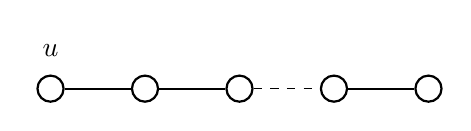
\begin{tikzpicture}[scale=1.2]
            \begin{scope}[every node/.style={circle,thick,draw}]
            \foreach \i in {1,...,5}
            {
                \ifthenelse{\i>1} {
                    \node (\i) at (\i,0) {}; } {
                    \node[label={$u$}] (\i) at (\i,0) {}; }
            }
            \end{scope}

            \foreach \i in {2,...,5}
            {
                \tikzmath{\im = int(\i-1);}
                \ifthenelse{\NOT \i=4} {
                    \path[-,thick,draw]
                    (\im) edge (\i); }{
                    \path[dashed,draw]
                    (\im) edge (\i); }
            }
            \end{tikzpicture}
        \end{subfigure}
        \begin{subfigure}{0.49\textwidth}
            \centering
            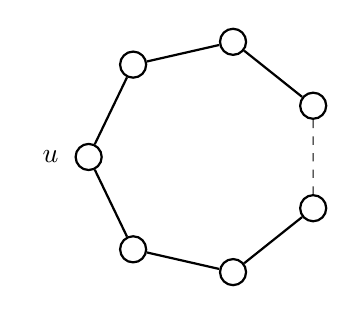
\begin{tikzpicture}[scale=0.6, rotate=180]
            \tikzmath{\n = 7; \r = 2.5;}
            \begin{scope}[every node/.style={circle,thick,draw}]
            \foreach \i in {1,...,\n}
            {
                \ifthenelse{\i>1} {
                    \node (\i) at ({360/\n * (\i - 1)}: \r) {}; } {
                    \node[label=left:{$u$}] (\i) at ({360/\n * (\i - 1)}: \r) {}; }
            }
            \end{scope}

            \foreach \i in {1,...,\n}
            {
                \tikzmath{\im = int(mod(\i,\n)+1);}
                \ifthenelse{\NOT \i=4} {
                    \path[-,thick,draw]
                    (\im) edge (\i); }{
                    \path[dashed,draw]
                    (\im) edge (\i); }
            }
            \end{tikzpicture}
        \end{subfigure}
        \caption{Prikazana sta grafa $P_n$ (levo) in $C_n$ (desno), za katera velja $\fms{(P_n)} = 1$ in $\fms{(C_n)}=2$.}
        \label{fig:fms-pot-cikel}
    \end{figure}
    Iščemo število hitrega mešanega iskanja za pot $P_n$ (na sliki~\ref{fig:fms-pot-cikel} levo). Recimo, da začnemo z enim iskalcem, ki ga na začetku postavimo v levo krajišče~$u$. Iskalec lahko zdrsi eno v desno, saj ima trenutno vozlišče samo eno okuženo povezavo, ki s tem postane preiskana. Tako lahko nadaljuje vsako potezo, saj je povezava levo od njega preiskana, desno od njega pa (edina) okužena. (Opazimo, da so povezave levo od iskalca nedosegljive za ubežnika, saj mu na poti stoji iskalec.) En iskalec je torej dovolj, da preiščemo cel graf, velja $\fms{(P_n)} = 1$.

    Kaj pa, če postavimo enega iskalca v vozlišče $u$ na ciklu $C_n$ (na sliki~\ref{fig:fms-pot-cikel} desno)? Ta ne more začeti drseti, saj ima dve okuženi povezavi. Recimo, da ga začnemo premikati po okuženih vozliščih gor. Potem povezave, ki jih je že obiskal, po definiciji niso preiskane, kar vidimo tudi iz tega, lahko ubežnik pride do njih po drugi polovici cikla. En iskalec torej ne bo dovolj, saj mu ubežnik lahko vedno pobegne ``malo naprej po ciklu''. Če pa dodamo še enega iskalca v vozlišče, sosednje $u$, je vmesna povezava preiskana. Zato lahko začne vsak iskalec drseti po ciklu v svojo smer, slej ko prej torej preiščeta vse povezave in s tem cel graf. Velja $\fms{(C_n)} = 2$.
\end{primer}

Opazimo lahko, da se vrednosti v primeru~\ref{prim:fms} ujemata z vrednostmi števila ničelne prisile za ti dve družini grafov. Pravzaprav lahko vidimo, da je pravilo, kdaj je vozlišče preiskano, na nek način ekvivalentno pravilu za spremembo barve vozlišča: iskalec zdrsi po povezavi (iz preiskanega vozlišča $u$ v okuženo vozlišče, ki postane preiskano) samo, če so vse ostale povezave neokužene oziroma preiskane -- podobno, kot črno vozlišče $u$ povzroči spremembo barve v nekem belem vozlišču samo, če so vsi ostali njegovi sosedi črne barve. Intuitivno se zdi, da sta števili morda povezani; brez dokaza navedimo
\begin{izrek}[{\cite[izrek 3.1]{fallat2016complexity}}]
    \label{izr:fms-je-zfs}
    Za poljuben graf $G$ velja $\fms{(G) = Z(G)}$.
\end{izrek}
\begin{posledica}
    \ZFOdl\ je $\NP$-poln.
\end{posledica}
\begin{proof}
     V~\cite{yang2013fast} je dokazano, da je problem hitrega mešanega iskanja (ali za dan graf $G$ velja $\fms{(G)} \leq k$) $\NP$-poln. Iz izreka~\ref{izr:fms-je-zfs} torej sledi $\NP$-polnost problema \ZFOdl.
\end{proof}

V~\cite{brimkov2017complexity} je obravnavana zahtevnost izračuna ožjega problema, \emph{povezane ničelne prisile}, pri kateri mora induciran graf nad vozlišči množice ničelne prisile tvoriti povezan graf.
\begin{definicija}
    Število povezane ničelne prisile je definirano kot
    \[ Z_c(G) = \min\{|Z| \mid Z \text{ množica ničelne prisile in } G[Z] \text{ povezan} \} \]
\end{definicija}
Iz definicij je razvidno, da velja $Z(G) \leq Z_c(G)$. V splošnem iz $\NP$-polnosti širšega problema ne sledi $\NP$-polnost ožjega, saj zoženje morda poenostavi problem. V primeru povezane ničelne prisile pa se izkaže, da je tudi ožji problem (njegova odločitvena različica) $\NP$-poln:
\begin{izrek}[{\cite[izrek 3]{brimkov2017complexity}}]
    Če \ZFOdl\ zožimo samo na tiste množice ničelne prisile, ki inducirajo povezan podgraf, je problem še vedno $\NP$-poln.
\end{izrek}
Poglejmo si hiter oris dokaza zgornjega izreka. Spomnimo se definicije $\NP$-polnosti~(\ref{def:np-poln}): veljati mora, da je odločitveni problem v $\NP$ in da lahko vsak problem iz $\NP$ v polinomskem času prevedemo na tega. Povezana različica \ZFOdl\ je v $\NP$, saj obstaja certifikat -- ta je kar množica ničelne prisile $Z$, velikosti manjše ali enake $k$ -- ki je polinomske dolžine glede na vhodne podatke ($O(n)$) in je preverljiv v polinomskem času (uporabimo algoritem~\ref{alg:preveri-zf-izboljsan} in BFS za preverjanje povezanosti induciranega podgrafa $G[Z]$).

Sedaj $\NP$-polnost dokažemo tako, da že znan $\NP$-poln problem \ZFOdl\ prevedemo na povezanega: vhodni podatek, graf $G = (V,E)$, modificiramo tako, da mu dodamo še eno vozlišče $v$, s katerim povežemo vsa vozlišča iz $V$, nato pa dodamo še dve vozlišči, ki ju povežemo z $v$. Nov graf označimo z $G'$. Sedaj trdimo, da ima $G$ množico ničelne prisile velikosti manjše ali enake~$k$ natanko tedaj, ko ima $G'$ povezano množico ničelne prisile velikosti manjše ali enake $k + 2$. Podrobnosti dokaza te ekvivalence so zapisane v~\cite{brimkov2017complexity}. Opazimo še, da je naša prevedba res polinomske časovne zahtevnosti glede na vhodne podatke \ZFOdl.

Poglejmo si še eno različico ničelne prisile, kjer za vhod dobimo utežen graf $G$.
Vsakemu vozlišču priredimo neko utež s pomočjo funkcije $w\colon V(G) \rightarrow \R$. Namesto velikosti $z$ množice ničelne prisile~$Z$ bomo sedaj upoštevali težo: $w(Z) = \sum_{i=1}^{z} w(u_i)$, število ničelne prisile sedaj definiramo kot
\[ Z(G, w) = \min\{ w(Z) \mid Z \text{ množica ničelne prisile} \} .\]

\begin{izrek}[\cite{aazami2008hardness}]
    Problem \ZFOdl\ je $\NP$-poln za ravninske grafe z utežmi, tudi če so uteži kvečjemu 0 ali 1.
\end{izrek}
Posledično sledi tudi $\NP$-polnost uteženega problema za splošne grafe. To ni presenetljivo, saj je \ZFOdl\ za neutežene grafe ožji problem (predstavljamo si lahko, da imajo vse uteži vrednosti 1), za katerega vemo, da je $\NP$-poln, torej mora tak biti tudi širši problem. Ker je bila $\NP$-polnost uteženega problema dokazana 8~let pred neuteženim, pa je dokaz ponovno narejen s pomočjo polinomske prevedbe že znanega $\NP$-polnega problema, usmerjenega Hamiltonskega cikla, na naš problem. (Da je problem v $\NP$, pa pokažemo enako, kot za primer povezane ničelne prisile.)

Avtor v~\cite[izrek~2.3.8]{aazami2008hardness} za utežen problem dokaže tudi, da je za poljuben fiksen $\epsilon > 0$ $\NP$-težko najti približek rešitve $Z(G,w)$ na $2^{\log^{1-\epsilon}n}$ natančno. \hl{TODO: katera osnova logaritma?} Če bi torej obstajal aproksimativen algoritem s tako konstanto, bi sledilo $\P = \NP$, zato pričakujemo, da takšni aproksimativni algoritmi ne obstajajo.

\subsection{Pregled algoritmov za specifične družine grafov}
%Greedy nekam?
%Kaj pa algoritem, ki vrne neko množico ničelne prisile? Npr.~začnemo z vsemi vozlišči, potem odstranimo vozlišča stopnje 1 etc ali kaj podobnega? Spet nekaj s path coveringom morda pomaga?

\section{Pregled ostalih rezultatov ničelne prisile}
V tem poglavju naredimo hiter pregled ostalih rezultatov, povezanih s pojmom ničelne prisile. V prvem podpoglavju se osredotočimo na boljše zgornje in spodnje meje za grafe, ki ustrezajo nekaterim pogojem glede največje in najmanjše stopnje vozlišča, v drugem podpoglavju pa si ogledamo, kako je ničelna prisila povezana z nekaterimi drugimi parametri na grafih, kot so  \hl{TODO}.

\subsection{Boljša zgornja in spodnja meja}
Poglejmo si posplošitev ničelne prisile, ki je bila uvedena v~\cite{amos2015kforcing} in s pomočjo katere so bile v~\cite{amos2015kforcing, gentner2018bounds} dokazane boljše zgornje meje za osnovno ničelno prisilo.
\begin{definicija}
    \emph{Število $k$-prisile} grafa $G$ za pozitivno celo število $k$, označimo $F_k(G)$, je velikost najmanjše take množice $Z \subseteq V$, da velja: če na začetku s črno pobarvamo vozlišča iz $Z$, ostala pa so bela, in upoštevamo pravilo, da črno vozlišče z največ $k$ belimi sosedi povzroči spremembo barve vseh teh, je po koncu postopka pobarvan cel graf $G$. Vse take množice $Z$, kjer je po koncu širjenje barve pobarvan cel graf, pravimo množice $k$-prisile.
\end{definicija}

Ničelna prisila je poseben primer $k$-prisile za $k=1$. Na podoben način kot~\eqref{eq:trv-spodnja-meja} lahko sklepamo spodnjo mejo za $k$-prisilo:
\begin{equation}
    F_k(G) \geq \min\{1, \delta - k + 1\} .
    \label{eq:kprisila-trv-spodnja-meja}
\end{equation}

Če imamo namreč graf z najmanjšo stopnjo $\delta$ in poskusimo sestaviti množico $k$-prisile velikosti $\delta - k$, za neko črno vozlišče $u$ torej vemo, da ima vsaj $\delta$ sosedov in da jih je pobarvanih največ $\delta - k - 1$, torej je najmanj $k + 1$ sosedov belih in širjenje barve se ne more začeti.

Poglejmo si vrednosti števila $k$-prisile za nekaj osnovnih družin grafov. Za pot očitno velja $F_k(P_n) = Z(P_n) = 1$, saj je to najmanjša možna velikost množice $k$-prisile. Za $k \geq 2$ je tudi za cikel dovolj, če začetna množica vsebuje samo eno vozlišče, saj ima to vozlišče dva bela soseda, ki za $k \geq 2$ oba postaneta črna, nato pa se širjenje barve nadaljuje kot pri ničelni prisili. Velja torej
\[ F_k(C_n) =
\begin{cases}
    2, & k = 1; \\
    1, & \text{sicer.}
\end{cases}
\]
Za polni graf pa velja $F_k(K_n) = n-k$, saj ima neko (vsako) črno vozlišče torej $k$ belih sosedov in jim spremeni barvo.

Očitno je neka množica $k$-prisile $Z$ tudi množica $(k+1)$-prisile: če lahko za začetno množico $Z$ s pravilom, da črno vozlišče s $k$ belimi sosedi spremeni barvo vsem tem, pobarvamo cel graf, ga lahko še toliko bolj, če ima lahko črno vozlišče iz pravila širjenja barve še enega belega soseda več. Vsaka množica $k$-prisile je tudi množica $(k+1)$-prisile, obratno pa seveda ni nujno res; ker iščemo minimum in je množic $k$-prisile torej manj, velja
\[ F_{k}(G) \geq F_{k+1}(G). \]
za nek graf $G$.

Navedimo zgornje meje za število $k$-prisile, dokazane v~\cite{amos2015kforcing}, in si poglejmo, kako se poenostavijo v primeru ničelne prisile.

\begin{izrek}{\cite[izrek 3.4]{amos2015kforcing}}
    Naj bo $k$ pozitivno celo število. Imejmo graf $G$ z $n \geq 2$ in naj za stopnje vozlišč velja $\Delta \geq k, \delta \geq 1$. Potem za število $k$-prisile velja naslednja zgornja meja
    \begin{equation}
        \label{eq:kprisila-zgornja-meja}
        F_k(G) \leq \frac{(\Delta - k + 1)n}{\Delta - k + 1 + \min\{\delta,k\}}
    \end{equation}
\end{izrek}

\begin{posledica}
    Naj bo $k$ pozitivno celo število. Imejmo graf $G$ z $n \geq 2$ in naj za najmanjšo stopnjo vozlišča velja $\delta \geq k$. Potem za število $k$-prisile velja naslednja zgornja meja
    \[ F_k(G) \leq \frac{(\Delta - k + 1) n}{\Delta + 1}, \]
    ki je tesna.
\end{posledica}
\begin{proof}
    Tesnost zgornje meje dobimo, če vzamemo polni graf $K_{\Delta + 1}$, $\Delta \geq k$, ki je $\Delta$-regularen graf (vsa vozlišča so stopnje $\Delta$). Če vstavimo, dobimo
    \[ F_k(K_{\Delta + 1}) \leq \frac{(\Delta - k + 1) (\Delta + 1)}{\Delta + 1} = \Delta - k +1, \]
    hkrati pa iz $\delta = \Delta$, $\Delta \geq k$ in~\eqref{eq:kprisila-trv-spodnja-meja} sledi
    \[ F_k(K_{\Delta + 1}) \geq \Delta - k +1, \]
    torej velja enakost in zgornja meja je tesna.
\end{proof}

\begin{posledica}
    Za graf $G$ z vsaj 2 vozliščema in najmanjšo stopnjo $\delta \geq 1$ (nimamo izoliranih vozlišč) za ničelno prisilo velja naslednja zgornja meja
    \begin{equation}
        \label{eq:zgornja-meja-zf}
        Z(G) = F_1(G) \leq \frac{\Delta}{\Delta + 1} n,
    \end{equation}
    ki je tesna za $K_{\Delta + 1}$ z $\Delta \geq 1$.
\end{posledica}

Za primera $k=1$ in $k=2$ pa obstaja še boljša meja, če predpostavimo povezanost grafa $G$. Graf je \emph{$k$-povezan}, če ima več kot $k$ vozlišč in ob odstranitvi poljubne podmnožice manj kot $k$ vozlišč preostanek inducira povezan podgraf.
\begin{izrek}{\cite[izrek 4.4]{amos2015kforcing}}
    Naj bo $k$ pozitivno celo število. Imejmo $k$-povezan graf $G$ z $n > k$ in $\Delta \geq 2$. Potem velja
    \begin{equation}
        \label{eq:kprisila-zgornja-meja-povezan}
        F_k(G) \leq \frac{(\Delta - 2)n + 2}{\Delta + k -2},
    \end{equation}
    meja je tesna.
\end{izrek}
Tesnost meje ponovno vidimo, če vzamemo graf $K_{\Delta + 1}$ z $\Delta \geq k$ in je $k=1$ ali $k=2$. Dobimo
\[  F_k(G) \leq \frac{(\Delta - 2)(\Delta + 1) + 2}{\Delta + k -2} = \frac{\Delta^2 - \Delta}{\Delta + k -2} = \frac{\Delta(\Delta - 1)}{\Delta + k -2}, \]
za $k = 1$ torej dobimo $\Delta$, kar vemo, da je enako $Z(K_{\Delta + 1})$, za $k = 2$ pa $\Delta - 1$, kar je enako $F_2(K_{\Delta + 1})$, meji sta v teh primerih tesni.

Če je $k \geq 3$, potem nam~\eqref{eq:kprisila-zgornja-meja} da boljšo mejo kot~\eqref{eq:kprisila-zgornja-meja-povezan}:
\begin{align*}
\frac{(\Delta - k + 1)n}{\Delta - k + 1 + \min\{\delta,k\}} &\leq \frac{(\Delta - 2)n}{\Delta - k + 1 + k}
\leq \frac{(\Delta - 2)n}{\Delta + 1} \leq \frac{(\Delta - 2)n}{\Delta + k - 2} \\
&\leq \frac{(\Delta - 2)n + 2}{\Delta + k - 2},
\end{align*}
pri čemer smo upoštevali trivialni neenakosti $1 - k \leq -2$ (pri prvi zgornji neenakosti) in $k - 2 \geq 1$ (pri tretji zgornji neenakosti) za $k \geq 3$ ter dejstvo, da iz $k$-povezanosti grafa sledi $\delta \geq k$ (v nasprotnem primeru bi poiskali vozlišče z minimalno stopnjo $\delta < k$, odstranili vse njegove sosede in dobili izolirano vozlišče, induciran podgraf preostanka ne bi bil povezan, torej bi imeli protislovje s predpostavko $k$-povezanosti).

\begin{posledica}
    Za povezan graf $G$ z $\Delta \geq 2$ velja
    \begin{equation}
        \label{eq:zgornja-meja-zf-povezan}
        Z(G) = F_1(G) \leq \frac{(\Delta - 2)n + 2}{\Delta - 1},
    \end{equation}
    meja je tesna za $K_{\Delta + 1}$ in $K_{\Delta, \Delta}$ za $\Delta \geq 2$.
\end{posledica}
\begin{proof}
    Tesnost meje za $K_{\Delta + 1}$ smo dokazali zgoraj. Za $K_{\Delta, \Delta}$ dobimo
    \[ Z(K_{\Delta, \Delta}) \leq \frac{(\Delta - 2)2\Delta + 2}{\Delta - 1} = \frac{2(\Delta^2 - 2 \Delta + 1)}{\Delta - 1} = \frac{2(\Delta- 1)^2}{\Delta - 1} = 2 (\Delta-1), \]
    iz trditve~\ref{trd:polni-dvodelni-graf} pa vemo, da je $Z(K_{\Delta, \Delta}) = 2\Delta - 2$, torej je meja tesna.
\end{proof}
\subsection{Povezave z drugimi grafovskimi parametri}


% Literatura:
% Primer navajanja na http://www.fmf.uni-lj.si/storage/24240/LiteraturaM.pdf,
% ampak bi moral stil poskrbeti za vse. Reference se uredijo po abecedi.
% Če nobena izbira izmed @book, @atricle,... ni ok, potem se lahko vse napiše v
% @misc pod note={} in deluje tako kot normalen LaTeX.
% Komentar v bib datoteki se naredi samo s parom { }
% Za urejanje literature avtor priporoča program Jabref, ki zna tudi avtomatsko
% okrajšati imena revij. Za pravilno sortiranje vnosov brez avtorja, uporabite
% polje key={ }, kot v primeru.
% V primeru napak ustvarite issue na GitHubu ali pišite na jure.slak@fmf.uni-lj.si.
\cleardoublepage                           % na desni strani
\phantomsection                            % da prav delujejo hiperlinki
\addcontentsline{toc}{section}{\bibname}   % dodajmo v kazalo
\bibliographystyle{fmf-sl}                 % uporabljen stil je v datoteki fmf-sl.bst, na voljo tudi angleška verzija
\bibliography{literatura}                 % literatura je v datoteki, definirani na začetku
% Za stvarno kazalo
%\cleardoublepage                           % na desni strani
%\phantomsection                            % da prav delujejo hiperlinki
%\addcontentsline{toc}{section}{\indexname} % dodajmo v kazalo
%\printindex

\end{document}
